\documentclass[11pt,a4paper]{article}
% arXiv source generated from paper/manuscript/manuscript.md with pandoc (natbib); not compiled in the authoring environment.
\usepackage[utf8]{inputenc}
\usepackage[T1]{fontenc}
\usepackage{lmodern}
\usepackage{amsmath,amssymb}
\usepackage{graphicx}
\usepackage{booktabs,longtable,array,calc}
\usepackage[margin=2.5cm]{geometry}
\usepackage[numbers,sort&compress]{natbib}
\usepackage{hyperref}
\hypersetup{colorlinks=true,linkcolor=blue!50!black,citecolor=blue!50!black,urlcolor=blue!50!black}
\providecommand{\real}[1]{#1}
\providecommand{\tightlist}{\setlength{\itemsep}{0pt}\setlength{\parskip}{0pt}}
\setlength{\emergencystretch}{3em}
\title{QCM frequency and dissipation estimation using DDS excitation, gain--phase detection and complex-admittance reconstruction}
\author{openQCM NEXT impedance-analysis working group\thanks{Author list and affiliations to be finalised.}}
\date{Draft v0.1 --- 2026-10-06}
\begin{document}
\maketitle
\begin{abstract}
Impedance analysis gives the resonance frequency and the half-bandwidth
of a quartz crystal microbalance (QCM) directly from the conductance
spectrum, but the vector network analysers that produce it are costly
and bulky. We describe and test a measurement method in which a direct
digital synthesiser sweeps a quartz sensor placed in a resistive voltage
divider, an AD8302 gain/phase detector returns the magnitude and the
\emph{unsigned} phase of the divider transfer function, and the complex
admittance of the sensor is reconstructed by exact inversion of the
divider. The detector's phase ambiguity is resolved where the phase
crosses zero and left unsigned where it does not, which the conductance
tolerates because it is even in the sign of the phase. The resonance
frequency \(f_\mathrm{res}\) and the half-bandwidth \(\Gamma\) are then
estimated either from the maximum and the half-height width of the
conductance or by fitting the phase-shifted Lorentzian of Johannsmann et
al.~We derive in closed form the bias of the simpler estimators for a
rotated resonance
(\(f_{G\max} - f_\mathrm{res} = \Gamma\tan(\varphi/2)\); half-height
width \(\Gamma\sqrt{1+2\tan^2(\varphi/2)}\)) and verify it on 45 sweeps.
On one instrument the rotation angle is \(\varphi = -8^\circ\) to
\(-27^\circ\) from the fundamental (5 MHz) to the 9th overtone, stable
to \(0.3^\circ\) between sweeps and to \(0.2\)--\(1.5^\circ\) between
air and liquid on overtones 3--9, and coincides with the board phase
obtained from an independent two-channel forward model: it is an
instrument property. Against the Kanazawa--Gordon prediction for water
and isopropanol at 25 °C, the air-to-liquid frequency shifts on
overtones 3--9 deviate by +52 to +92 \% with the magnitude channel
alone, by +20 to +30 \% with the maximum of the reconstructed
conductance and by −1.4 to +8.2 \% with the phase-shifted Lorentzian,
while the bandwidth shifts are within ±7.4 \% with the half-height width
and within −3.9 to +9.3 \% with the fit. The Newtonian ratio
\(|\Delta f|/\Delta\Gamma\) is 0.98--1.08 with the fit against
1.17--1.34 with the conductance maximum. The fundamental deviates by +29
to +37 \% in bandwidth with every estimator and is attributed to the
sensor mounting. On a second instrument and crystal, measured in 2024 in
air, water and glucose solutions (5, 7.5 and 10 \% w/v), the same
estimators give a Newtonian ratio of 1.20--1.41 (conductance maximum)
against 1.01--1.16 (fit) on overtones 3--9 in all four liquids, a water
frequency shift of +20 to +36 \% against +6 to +13 \% over the theory, a
rotation angle that agrees with the first instrument within 1--3° on
four of five overtones but is not monotonic in frequency, and a
fundamental that follows the theory (bandwidth +4 to +7 \%). A forward
model with a board phase acting on the measured transfer function shows
that the rotated-Lorentzian correction is exact only when the motional
resistance is large compared with the divider resistor, which holds in
liquid, and quantifies the residual. All raw data and analysis scripts
are released.
\end{abstract}
\noindent\textbf{Keywords:} quartz crystal microbalance; QCM-D; impedance analysis; AD8302; gain--phase detector; direct digital synthesis; phase-shifted Lorentzian; Kanazawa--Gordon; open-source instrumentation.

\hypertarget{introduction}{%
\section{Introduction}\label{introduction}}

A quartz crystal microbalance (QCM) reports the mass and the mechanical
properties of what touches its surface through two numbers: the shift of
its resonance frequency, \(\Delta f\), and the shift of its
half-bandwidth, \(\Delta\Gamma\), or equivalently of the dissipation
factor \(D = 2\Gamma/f_\mathrm{res}\)
\citep{Sauerbrey1959, KanazawaGordon1985AC, Johannsmann2021}. The second
number is what distinguishes a rigid film from a viscoelastic one and a
Newtonian liquid from a structured one, and it is the one that simple
oscillator circuits do not provide: an oscillator locks on one frequency
and reports one number, and its definition of that frequency moves with
the load \citep{Arnau2008, RodriguezPardo2004}. Ring-down (QCM-D)
instruments obtain \(D\) from the decay of the free oscillation
\citep{Rodahl1995} and impedance analysers obtain \(f_\mathrm{res}\) and
\(\Gamma\) from a fit of the admittance trace
\citep{Martin1991, Johannsmann2021, JohannsmannReviakine2024}. Both are
commercial, bench-sized instruments.

Between the oscillator and the network analyser sits a class of compact
sweep-based instruments that excite the crystal with a direct digital
synthesiser (DDS) and record the response with a scalar detector. The
open-source openQCM family
\citep{openQCMQ1, openQCMNEXT, Horst2022, Munoz2023} uses an AD9851 DDS,
a voltage divider formed by the sensor and a series resistor, and an
AD8302 gain/phase detector \citep{AD8302Datasheet}, which outputs two DC
voltages proportional to the logarithmic magnitude ratio and to the
\emph{modulus} of the phase difference between its inputs. In its
production software, such an instrument reads the resonance frequency as
the maximum of the magnitude curve and a ``dissipation'' as the width of
that curve a fixed number of decibels below the maximum. The magnitude
of a divider transfer function is not the conductance of the crystal:
its peak sits between the series and the parallel resonance and moves
with the static capacitance and the load, and its width has no
counterpart in the theory \citep{Johannsmann2021}. We show below that in
liquid this estimator overshoots the Kanazawa--Gordon frequency shift by
50--90 \% on the overtones.

The phase channel of the AD8302 is what makes a vector measurement
possible, and it is what has been left unused: the detector cannot tell
the sign of the phase difference, its output folds at zero, and it
carries an offset. This article asks whether the two detector outputs,
inverted exactly through the known divider, yield a complex admittance
good enough to apply the standard QCM impedance-analysis estimators, and
which estimator should then be used. The phase-shifted Lorentzian we end
up recommending is not new --- it is the fit function of Johannsmann and
co-workers \citep{Johannsmann2021, Leppin2020, JohannsmannReviakine2024}
and the same mathematics as the ``background phase'' of
microwave-resonator circle fits
\citep{KajfezHwan1984, PetersanAnlage1998, Khalil2012, Probst2015} ---
and neither are the hardware blocks. What we believe is new is the chain
and its test: exact complex-admittance reconstruction from a gain/phase
detector in a resistive divider, a treatment of the detector's phase
ambiguity that uses the resonance itself, closed-form expressions for
the bias of the conductance-maximum and half-height estimators when the
resonance is rotated, an interpretation of the fitted rotation angle as
the board phase of the detector chain, and a quantitative comparison of
three estimators on the same sweeps against Kanazawa--Gordon on five
overtones in two liquids, with raw data released.

The contributions are therefore: (i) the exact inversion
\(M = |Z_q + R_{17}|\), \(R_q = M\cos\phi - R_{17}\),
\(X_q = -M\sin\phi\), \(Y_q = 1/Z_q\) from the AD8302 outputs, with the
constants verified against the schematic and the data sheet; (ii) a
documented treatment of the folded, offset, unsigned phase reading, and
the observation that the conductance --- hence \(f_\mathrm{res}\) and
\(\Gamma\) --- needs only the unsigned phase but is sensitive to its
offset; (iii) the closed forms
\(f_{G\max} = f_\mathrm{res} + \Gamma\tan(\varphi/2)\),
\(\Gamma_\mathrm{hh} = \Gamma\sqrt{1 + 2\tan^2(\varphi/2)}\),
\(f_\mathrm{mid} = f_\mathrm{res} + 2\Gamma\tan(\varphi/2)\) for the
rotated Lorentzian, and their verification; (iv) the finding that the
rotation angle is an instrument constant equal to the board phase; (v)
the experimental ranking of the estimators against Kanazawa--Gordon,
including the separation of what complex-admittance reconstruction buys
from what the rotation correction buys; (vi) a forward model that bounds
the validity of the rotated-Lorentzian correction for this front end.

\hypertarget{measurement-principle-and-hardware}{%
\section{Measurement principle and
hardware}\label{measurement-principle-and-hardware}}

The sensor is a 5 MHz AT-cut quartz crystal (openQCM NEXT holder, gold
electrodes, 14 mm blank) operated on its fundamental and 3rd, 5th, 7th
and 9th overtones (5--45 MHz). The instrument (openQCM NEXT, board 1920)
comprises an AD9851 DDS clocked at 125 MHz (its specified maximum at 3.3
V), an LC reconstruction filter and a level-setting driver, the crystal
as the series element of a voltage divider loaded by
\(R_{17} = 52.3\ \Omega\) to ground, an AD8302 gain/phase detector whose
input A reads the node across \(R_{17}\) and whose input B reads the
drive through a resistive attenuator
(\(K = (R_{11}+R_{19})/R_{19} = 10.419\), 20.356 dB), two output buffers
(gains 2 and 1.5) and the 12-bit ADC of a Teensy 4.0, which averages 500
readings per frequency point and streams the pair of counts to the host
(Fig. 1). A Peltier element holds the sensor at a set temperature (25.00
°C here). The firmware sweeps 18 001 points at 1 Hz step over a window
of −12 kHz/+6 kHz around the previous resonance of each overtone; a
sweep takes about 1.8 s per overtone.

\begin{figure}
\centering
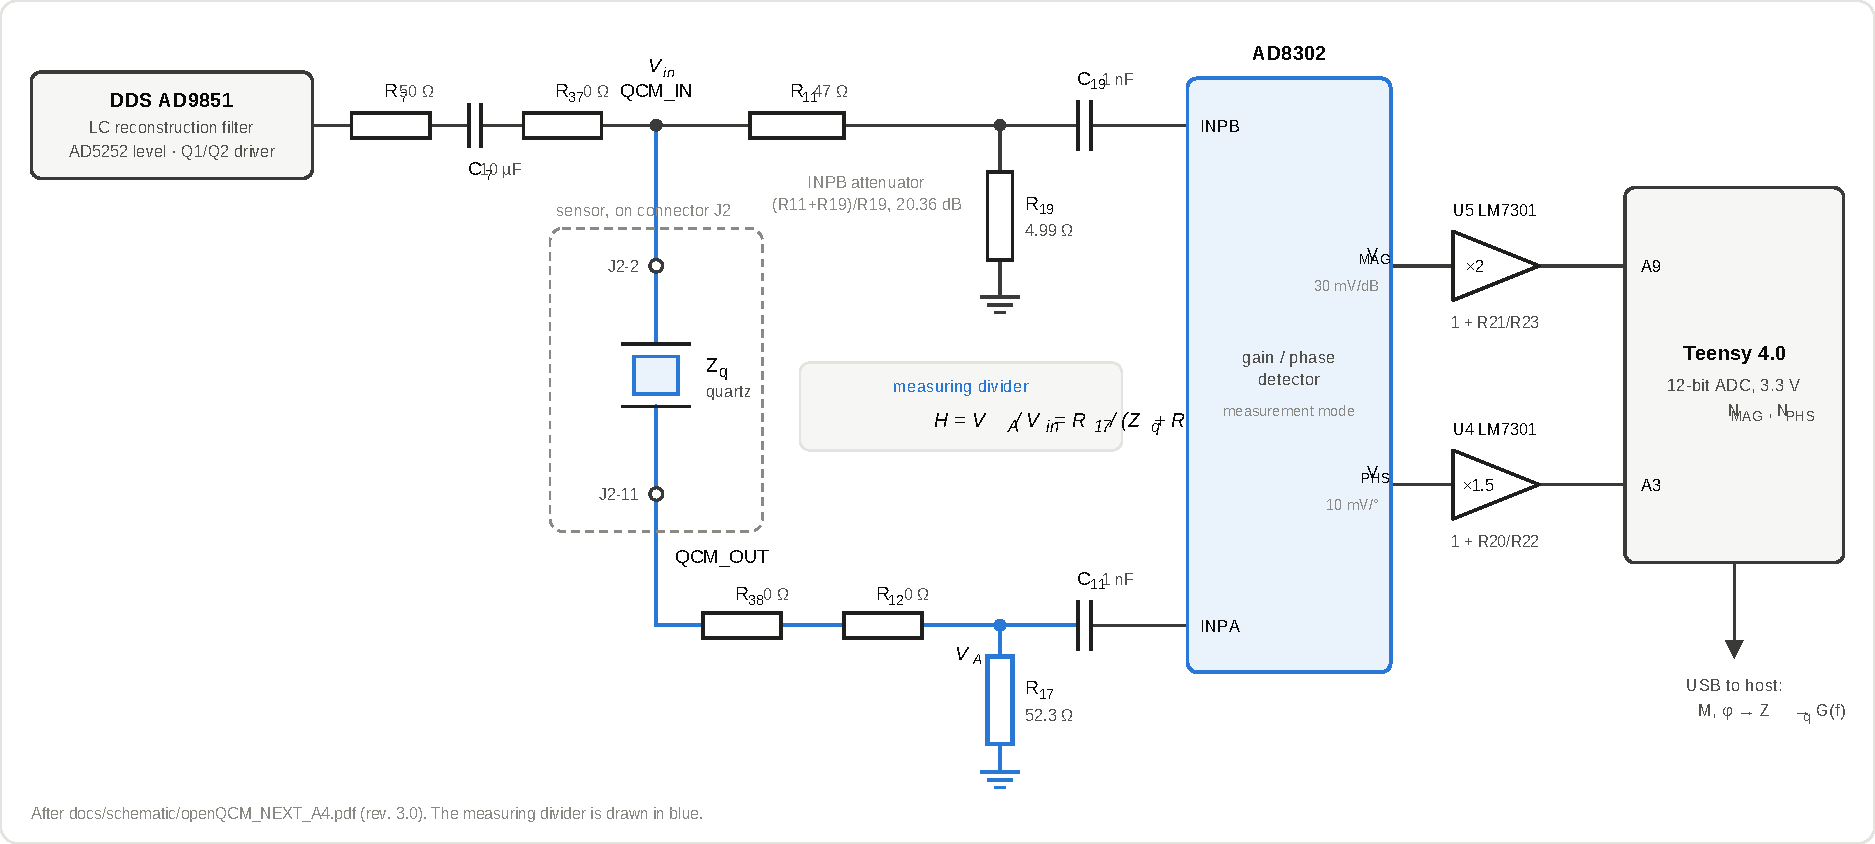
\includegraphics[width=\linewidth]{figures/fig01_measurement_circuit.pdf}
\caption{Fig. 1. Measurement circuit: the quartz sensor in a divider
with \(R_{17}\), read by the AD8302 gain/phase detector; drawn after the
openQCM NEXT schematic (repository figure).}
\end{figure}

The host software (Python) converts the counts to the detector voltages
\(V_\mathrm{MAG}\) and \(V_\mathrm{PHS}\), removes the attenuator from
\(V_\mathrm{MAG}\), smooths both channels (Savitzky--Golay, 51 points,
order 3, followed by a smoothing spline, \(s = 10^{-3}\), on the 1 Hz
grid), reconstructs \(G(f)\) and \(B(f)\) as described in Section 3 and
estimates \(f_\mathrm{res}\) and \(\Gamma\) as described in Section 4.
The datalog records, per sweep and overtone, \(f_\mathrm{res}\) and
\(D = 2\Gamma/f_\mathrm{res}\). On request the software also writes the
raw per-point triplets (frequency, \(V_\mathrm{MAG}\),
\(V_\mathrm{PHS}\)), which are the input of every result in this paper.

\hypertarget{complex-admittance-reconstruction}{%
\section{Complex-admittance
reconstruction}\label{complex-admittance-reconstruction}}

\hypertarget{divider-and-detector-laws}{%
\subsection{Divider and detector
laws}\label{divider-and-detector-laws}}

The divider transfer function is

\[H(f) = \frac{V_A}{V_\mathrm{in}} = \frac{R_{17}}{Z_q(f) + R_{17}},\qquad \frac{V_\mathrm{INPA}}{V_\mathrm{INPB}} = K\,H(f). \tag{1}\]

The AD8302 obeys, with \(V_\mathrm{CP} = 0.900\) V
\citep{AD8302Datasheet},

\[V_\mathrm{MAG} = V_\mathrm{CP} + 0.600\ \mathrm{V}\cdot\log_{10}\frac{|V_\mathrm{INPA}|}{|V_\mathrm{INPB}|},\qquad V_\mathrm{PHS} = V_\mathrm{CP} - 0.010\ \mathrm{V}/^\circ\cdot\left(|\angle V_\mathrm{INPA} - \angle V_\mathrm{INPB}| - 90^\circ\right). \tag{2}\]

After the attenuator is removed
(\(V_\mathrm{MAG} \leftarrow V_\mathrm{MAG} - 0.030\cdot 20\log_{10}K = V_\mathrm{MAG} - 0.6107\)
V; the 0.36 dB by which the attenuator differs from one decade is 4 \%
on \(M\) and up to 22 \% on the motional resistance in air, so the
constant must be computed, not rounded), the magnitude of the sum
\(Z_q + R_{17}\) follows from Eqs. (1)--(2):

\[M \equiv |Z_q + R_{17}| = R_{17}\,10^{(V_\mathrm{CP} - V_\mathrm{MAG})/0.6}. \tag{3}\]

The phase of the divider is \(\angle H = -\angle(Z_q + R_{17})\).
Writing \(\phi = \angle H\), so that \(Z_q + R_{17} = M e^{-j\phi}\),

\[R_q = M\cos\phi - R_{17},\qquad X_q = -M\sin\phi, \tag{4}\]

\[G = \frac{R_q}{R_q^2 + X_q^2} = \frac{M\cos\phi - R_{17}}{(M\cos\phi - R_{17})^2 + (M\sin\phi)^2},\qquad B = \frac{-X_q}{R_q^2 + X_q^2}. \tag{5}\]

Equations (3)--(5) were derived independently of the instrument code and
agree with it to machine precision; a short (\(Z_q = 0\)) gives
\(M = R_{17}\) and \(\phi = 0\), as required. The inversion is
ill-conditioned near the series resonance of a lightly damped crystal,
where \(X_q \to 0\) and \(R_q = M\cos\phi - R_{17}\) is a difference of
close numbers: a relative error \(k - 1\) on \(M\) propagates to \(R_m\)
as \((k-1)(1 + R_{17}/R_m)\), i.e.~amplified 2.5× in air
(\(R_m \approx 36\ \Omega\) at the fundamental) and not at all in liquid
(\(R_m \approx 1\ \mathrm{k}\Omega\)). The frequency and bandwidth
estimates of Section 4, which depend on the \emph{shape} of \(G(f)\),
are much less sensitive to the magnitude scale (Section 6.8).

\hypertarget{the-phase-reading-fold-offset-sign}{%
\subsection{The phase reading: fold, offset,
sign}\label{the-phase-reading-fold-offset-sign}}

The detector returns the modulus of the phase difference. The reading in
degrees, \(r = (1.8\ \mathrm{V} - V_\mathrm{PHS})/0.010\) V, follows the
model

\[r(f) = |\phi(f) + \phi_b| - \delta, \tag{6}\]

in which \(\phi_b\) is a phase of the board and cabling that enters
\emph{inside} the modulus and \(\delta\) is a voltage offset of the
phase channel that enters \emph{outside} it. Two regimes occur (Fig. 2).
For a lightly damped crystal (air) the argument of the modulus crosses
zero near the series resonance; the reading has a V-shaped minimum
(``fold'') whose vertex value is \(-\delta\) exactly, so the offset is
\emph{measured} by the fold, and the sign of the phase is restored by
negating the branch past the vertex. For a damped crystal (water,
isopropanol, \(n \ge 3\) here) the static capacitance keeps the phase
away from zero, the reading has a smooth minimum tens of degrees above
zero, there is no fold, \(\delta\) is not identifiable from the sweep,
and the reading is taken as the signed phase with \(\phi_b - \delta\)
left in it. The instrument decides between the two regimes from how
close the reading's peak gets to zero relative to its off-resonance
baseline (depth \(\ge 0.88\)) and from the position of that peak
relative to the conductance maximum (within \(5\Gamma\)); the decision
is latched over two sweeps. This rule is an implementation detail
calibrated on this board, and we report its one observed fragility in
Section 6.9.

\begin{figure}
\centering
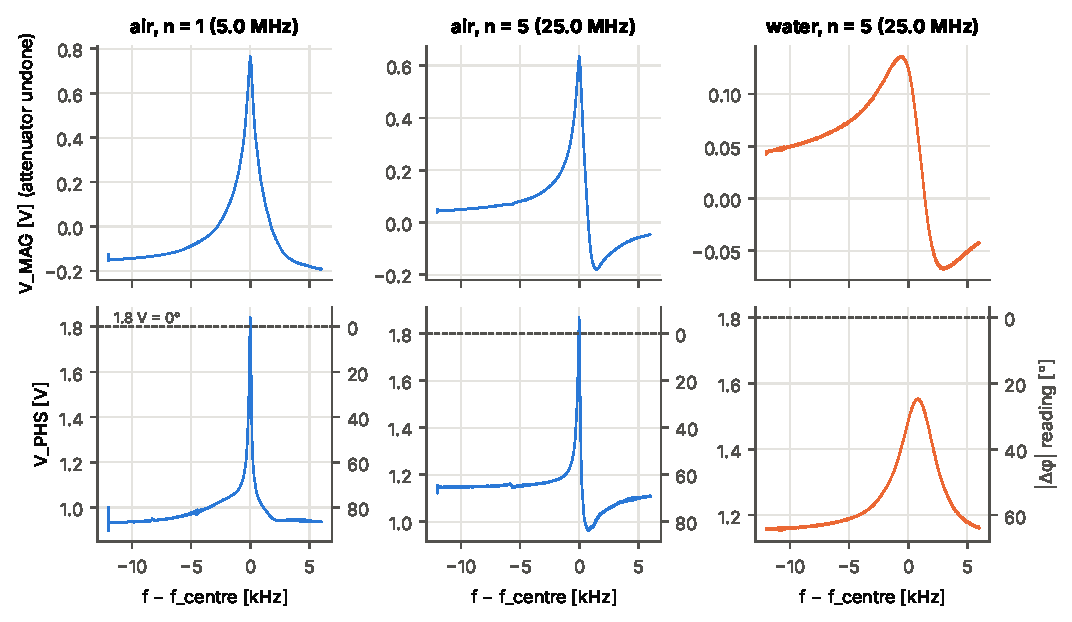
\includegraphics[width=\linewidth]{figures/fig02_raw_sweeps.pdf}
\caption{Fig. 2. Raw detector voltages for the fundamental and the 5th
overtone in air and for the 5th overtone in water (board 1920,
2026-09-11). Right axis: the unsigned phase reading
\(|\Delta\phi| = (1.8\ \mathrm{V} - V_\mathrm{PHS})/10\ \mathrm{mV}\).
In air the reading folds at zero (and overshoots it, the signature of
the offset \(\delta\)); in water it does not reach zero.}
\end{figure}

The conductance (5) depends on \(\phi\) only through \(\cos\phi\) and
\(\sin^2\phi\): it is even in the sign of the phase. The susceptance is
odd. Hence \(G(f)\), and with it \(f_\mathrm{res}\) and \(\Gamma\), can
be computed from the \emph{unsigned} reading on every load, while
\(B(f)\) and the admittance locus need the sign and are correct only
where a fold identifies it. Evenness in the sign does not extend to the
offset: \(G(\phi + \delta) \ne G(\phi)\), and an uncorrected \(\delta\)
of a few degrees distorts the peak shape --- it is one of the two
quantities that the rotation angle of Section 4.2 absorbs on damped
loads (Section 6.7). Figure 3 shows \(G\), \(B\) and the locus \(B(G)\)
for the three cases of Fig. 2.

\begin{figure}
\centering
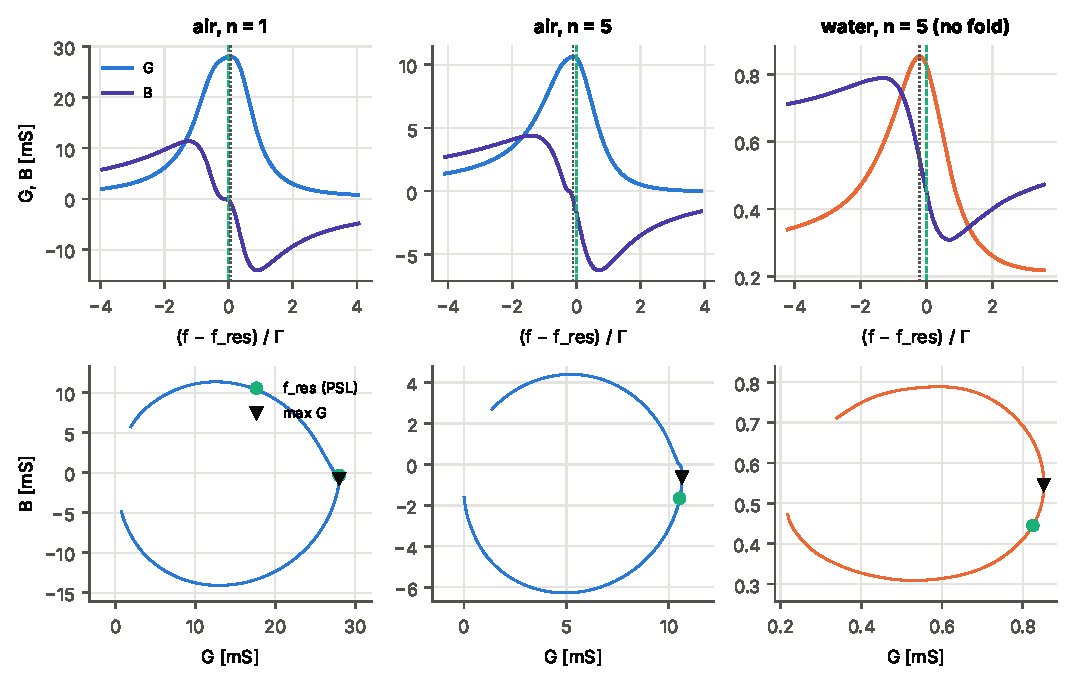
\includegraphics[width=\linewidth]{figures/fig03_G_B_locus.pdf}
\caption{Fig. 3. Reconstructed conductance and susceptance (top) and
admittance locus (bottom) on \(\pm4\Gamma\) around the resonance for the
sweeps of Fig. 2. Dotted: the maximum of \(G\); dashed/marker:
\(f_\mathrm{res}\) from the phase-shifted Lorentzian. The maximum of
\(G\) sits below \(f_\mathrm{res}\) and the locus is rotated with
respect to the \(G\) axis.}
\end{figure}

\hypertarget{resonance-parameter-estimation}{%
\section{Resonance parameter
estimation}\label{resonance-parameter-estimation}}

\hypertarget{conductance-maximum-and-half-height-width}{%
\subsection{Conductance maximum and half-height
width}\label{conductance-maximum-and-half-height-width}}

The standard estimator of the instrument takes \(f_{G\max}\), the
frequency of the sample where \(G\) is maximum on the 1 Hz grid, and the
half-height half width \(\Gamma_\mathrm{hh} = (f_+ - f_-)/2\), where
\(f_\pm\) are the linearly interpolated crossings of \(G - G_0\) with
half its maximum and \(G_0\) is the mean of the first 100 samples of the
sweep (an off-resonance baseline for a window sized for air). Then
\(D = 2\Gamma_\mathrm{hh}/f_{G\max}\). The midpoint \((f_+ + f_-)/2\) is
a second frequency estimator that costs nothing.

\hypertarget{the-phase-shifted-lorentzian-and-why-the-conductance-maximum-is-biased}{%
\subsection{The phase-shifted Lorentzian and why the conductance
maximum is
biased}\label{the-phase-shifted-lorentzian-and-why-the-conductance-maximum-is-biased}}

Near a resonance the motional admittance is
\(Y_m \propto 1/(\Gamma - j\Delta)\) with
\(\Delta = f_\mathrm{res} - f\) \citep[Eqs. 9--10]{Johannsmann2021}. A
calibration error that multiplies the admittance by a complex constant
\(e^{j\varphi}\) --- a residual phase of the measurement chain ---
rotates the resonance circle about its offset and gives

\[G(f) = G_\mathrm{max}\Gamma\,\frac{\Gamma\cos\varphi - \Delta\sin\varphi}{\Delta^2 + \Gamma^2} + G_\mathrm{off},\qquad B(f) = G_\mathrm{max}\Gamma\,\frac{\Gamma\sin\varphi + \Delta\cos\varphi}{\Delta^2+\Gamma^2} + B_\mathrm{off}. \tag{7}\]

This is the phase-shifted Lorentzian of Johannsmann et al. \citep[Eq.
13]{Johannsmann2021} in the rotation form; as printed there the \(G\)
line carries \(+\Delta\sin\varphi\), which with a common \(\varphi\) in
both lines is not a single rotation --- fitting \(G\) alone, the two
conventions differ only in the sign of \(\varphi\), and we quote
\(\varphi\) with the sign of Eq. (7) (negative on this board). The
dispersive term \(-\Delta\sin\varphi/(\Delta^2 + \Gamma^2)\) is
antisymmetric about \(f_\mathrm{res}\) and skews the peak. Setting
\(dG/d\Delta = 0\) gives
\(\sin\varphi\,\Delta^2 - 2\Gamma\cos\varphi\,\Delta - \Gamma^2\sin\varphi = 0\),
whose maximum is at \(\Delta = -\Gamma\tan(\varphi/2)\):

\[f_{G\max} = f_\mathrm{res} + \Gamma\tan\frac{\varphi}{2}, \tag{8}\]

so with \(\varphi < 0\) the maximum lies below the resonance by 0.07 Γ
at −8° and 0.25 Γ at −28°. The peak height is
\((G_\mathrm{max})\cos^2(\varphi/2)\) above \(G_\mathrm{off}\), and
solving for the half-height crossings (\(c = \cos^2(\varphi/2)\)) gives
\(\Delta_\pm = \Gamma[-\sin\varphi \pm \sqrt{c(2-c)}]/c\), hence

\[\Gamma_\mathrm{hh} = \Gamma\sqrt{1 + 2\tan^2\frac{\varphi}{2}},\qquad f_\mathrm{mid} = f_\mathrm{res} + 2\Gamma\tan\frac{\varphi}{2}: \tag{9}\]

the half-height width over-estimates \(\Gamma\) by 0.5 \% at −8° and 6
\% at −28°, and the midpoint is biased twice as much as the maximum, in
the same direction. Equations (8)--(9) were checked on noise-free model
curves to the 1 Hz grid (Supplementary table
\texttt{closed\_forms\_check.csv}). A \emph{symmetric} Lorentzian fitted
to a rotated one has no closed-form bias; numerically its centre is
displaced by 1.3--2.1 \(\Gamma\tan(\varphi/2)\) with a constant
background and by ≈1.25 \(\Gamma\tan(\varphi/2)\) with a linear
background, in the same direction as the maximum.

\hypertarget{fitting}{%
\subsection{Fitting}\label{fitting}}

The five parameters
\((G_\mathrm{max}, f_\mathrm{res}, \Gamma, \varphi, G_\mathrm{off})\) of
the \(G\) line of Eq. (7) are fitted to the smoothed \(G(f)\) by
Levenberg--Marquardt on the window
\(|f - f_{G\max}| \le 3\Gamma_\mathrm{hh}\), seeded with \(f_{G\max}\),
\(\Gamma_\mathrm{hh}\), \(\varphi = 0\) and \(G_\mathrm{off} = \min G\);
frequencies are scaled to kHz about the seed and conductances to mS so
that the Jacobian is well conditioned. The fit is accepted if it
converges, \(f_\mathrm{res}\) lies inside the window,
\(0.3 \le \Gamma/\Gamma_\mathrm{hh} \le 3\), \(|\varphi| \le 60^\circ\)
and the rms residual is below 5 \% of the range of \(G\) on the window;
otherwise the instrument falls back to the estimator of Section 4.1 and
logs the reason. \(D = 2\Gamma/f_\mathrm{res}\). The same code path
serves the instrument and the offline analysis; the analysis of this
paper uses an independent re-implementation from the equations above,
which reproduces the instrument's regression values to all printed
digits on the 45 sweeps.

\hypertarget{experimental-methods}{%
\section{Experimental methods}\label{experimental-methods}}

\textbf{Sensor and instrument.} 5 MHz AT-cut quartz (openQCM NEXT
sensor), gold electrodes, in the openQCM NEXT cell; instrument board
1920, DDS clock 125 MHz, firmware 0.1.5c, host software of the
\texttt{impedance-analysis} branch at commit \texttt{37fce4b}. Sensor
temperature 25.00 °C (Peltier; logged 24.93--25.00 °C, 25.00 °C on every
plateau). The liquid temperature was not measured (see Section 7).

\textbf{Protocol (2026-09-11).} Air, then deionised water, then
isopropanol poured into the cell in sequence, one acquisition of 75 min;
overtones 1, 3, 5, 7, 9 swept in turn, −12 kHz/+6 kHz at 1 Hz, 500 ADC
readings per point. Three raw sweep sets per liquid were copied during
the plateaus (air 12:25, 12:46, 12:50; water 12:57, 13:08, 13:15;
isopropanol 13:20, 13:24, 13:30), 45 sweeps in all. A second, shorter
run on the same board and sensor (2026-09-10, air → isopropanol → water,
23 min) provides a replicate of the datalog comparison, and five air
sweeps of 2026-09-03 (same board class, 125 MHz clock) a second day for
the rotation angle.

\textbf{Second dataset (2024-05-29).} A second openQCM NEXT, with a
second 5 MHz sensor, was measured two years earlier with the production
software and firmware 0.1.5: air, deionised water, then glucose
solutions of 5, 7.5 and 10 \% w/v poured in sequence, three raw sweep
sets per phase on overtones 1--9 (75 sweeps), same window and step. The
board and its DDS clock, the sensor and the liquid temperature were not
recorded (sensor temperature 24.95--25.02 °C in the datalog); no
open/short/load sweep of that board exists; the preparation method and
the purity of the glucose are to be confirmed by the operator
{[}placeholder: supplier, grade, weighing, water{]}. The raw files of
that software hold the two channels as instrument units --- column 2 is
\((V_\mathrm{MAG,uncomp.} - 0.9\ \mathrm{V})/0.030\), column 3 is
\(90^\circ - |\Delta\phi|\) --- and were converted to volts with the
attenuator removed (\(V_\mathrm{MAG} = 0.9 + 0.030\,c_2 - 0.6107\) V,
\(V_\mathrm{PHS} = 0.9 + 0.010\,c_3\) V). The software of 2024 also
wrote a second family of files that carry the same two channels with the
wrong attenuator constant (0.600 V); they were verified to be identical
to the converted raw files to \(2\times10^{-16}\) and excluded. The
firmware of 2024 has the same sweep-average carry-over as 0.1.5c
(below). The dataset is archived with its datalog in
\texttt{research/glucose-2024-05-29/}. Glucose is a liquid for which we
use no tabulated \(\rho\eta\): only the Newtonian ratio and the ratio
\(\rho\eta/(\rho\eta)_\mathrm{water} = (\Delta f/\Delta f_\mathrm{water})^2\)
from the air-referenced shifts are compared.

\textbf{Firmware correction.} Firmware versions up to 0.1.5c did not
reset the per-point sums, so each printed point carried 1/500 of the
previous one (+0.2 \% on the counts). The recursion is exact and was
undone offline (\(m_i = v_i - v_{i-1}/500\)); every result was computed
with and without the correction. It changes \(f_\mathrm{res}\) and
\(\Gamma\) by ≤2 Hz on 44 of 45 sweeps of 2026 and the error summaries
by ≤2 percentage points; the exception is discussed in Section 6.9. On
the 75 sweeps of 2024 it changes \(f_\mathrm{res}\) by ≤4 Hz, \(\Gamma\)
by ≤1 Hz and \(\varphi\) by ≤0.2°. Uncorrected values are reported
unless stated.

\textbf{Processing.} All estimators run on the same smoothed \(G(f)\)
(Section 2). Estimators: (M) magnitude only --- maximum of the divider
ratio in dB on the same grid, with its −3 dB full width where it exists
inside the window (the production software's −0.3 dB width is logged by
the instrument and reported from the datalog); (A) maximum of \(G\) and
half-height half width (Section 4.1); (MP) midpoint of the half-height
crossings; (S) symmetric Lorentzian with constant background (4
parameters) and with linear background (5); (P) phase-shifted Lorentzian
(Section 4.3); (C) for reference, the Butterworth--Van Dyke
admittance-circle fit of the repository's offline tool, on \(G + jB\).
Shifts are liquid minus air for the same estimator, mean of three
sweeps; their standard deviation is the quadrature sum of the two
replica standard deviations.

\textbf{Theory.} Kanazawa--Gordon in the small-load form normalised to
the fundamental \(f_F\) \citep{KanazawaGordon1985AC, Johannsmann2021}:
\(\Delta f_n = -\sqrt{n}\,f_F^{3/2}\sqrt{\rho\eta/(\pi\rho_q\mu_q)}\),
\(\Delta\Gamma_n = -\Delta f_n\), with \(\rho_q = 2648\) kg m\(^{-3}\),
\(\mu_q = 2.947\times10^{10}\) Pa, \(f_F = 5\,004\,596\) Hz (air), water
\(\rho = 997.05\) kg m\(^{-3}\), \(\eta = 0.890\) mPa s and isopropanol
\(\rho = 781.0\) kg m\(^{-3}\), \(\eta = 2.038\) mPa s at 25 °C, giving
673.6 \(\sqrt n\) Hz and 901.5 \(\sqrt n\) Hz. Error metrics:
\(\epsilon_f = \Delta f/\Delta f_\mathrm{KG} - 1\),
\(\epsilon_\Gamma = \Delta\Gamma/\Delta\Gamma_\mathrm{KG} - 1\) and the
Newtonian ratio \(\rho_N = |\Delta f|/\Delta\Gamma\), whose prediction
(unity) does not depend on \(\rho\eta\) or on temperature.

\textbf{Reproducibility.} Raw sweeps
(\texttt{research/air-ipa-water-1920-2026-09-11/data/sweep\_dumps\_2026-09-11.npz},
\texttt{research/glucose-2024-05-29/data/sweep\_raw\_2024-05-29.npz}),
datalogs, the analysis package (\texttt{paper/analysis/}:
\texttt{qcmchain.py}, \texttt{run\_estimators.py},
\texttt{run\_shifts.py}, \texttt{run\_datalogs.py},
\texttt{run\_bias\_theory.py}, \texttt{run\_forward\_model.py},
\texttt{run\_glucose.py}, \texttt{make\_figures.py}) and all result
tables are in the repository; every figure lists its source and
parameters in \texttt{results/figure\_provenance.md}.

\hypertarget{results}{%
\section{Results}\label{results}}

\hypertarget{raw-sweeps-and-reconstructed-admittance}{%
\subsection{Raw sweeps and reconstructed
admittance}\label{raw-sweeps-and-reconstructed-admittance}}

Figure 2 shows the detector outputs and Fig. 3 the reconstructed
spectra. In air the divider ratio at resonance is −4.5 dB (fundamental)
to −14 dB (9th) with 16--32 dB of contrast; in liquid the whole sweep
lies at −22 to −37 dB with 1.6--14 dB of contrast, against a specified
AD8302 range of ±30 dB. The phase reading folds in air on every overtone
(vertex −0.6° to −6.9°, i.e.~\(\delta\) = +0.6° to +6.9° after sign) and
on the fundamental in liquid; on \(n \ge 3\) in liquid its minimum stays
9--45° above zero. The reconstructed \(G(f)\) peaks at 10.8 mS (air,
5th) and 0.4--1.6 mS (liquids); \(B(f)\) has the dispersive shape
expected for a resonance and the locus \(B(G)\) is a circle to 1--7 \%
of its radius in air and 5--18 \% in liquid, visibly rotated with
respect to the \(G\) axis.

\hypertarget{symmetric-against-phase-shifted-lorentzian}{%
\subsection{Symmetric against phase-shifted
Lorentzian}\label{symmetric-against-phase-shifted-lorentzian}}

Figure 4 shows both fits and their residuals on three sweeps. The
symmetric Lorentzian (with linear background) leaves the same S-shaped
residual in every one of the 45 sweeps --- negative below the peak,
positive above, reversing one width out --- with an rms of 2.0--3.5 \%
of the range of \(G\) in liquid and 3.4--4.1 \% in air; the
phase-shifted Lorentzian leaves 0.15--0.65 \% in liquid and 1.0--2.7 \%
in air, where the remaining feature is a 20--50 Hz wide bump at the top
of the peak caused by the rounding of the detector's phase fold, which
does not move \(f_\mathrm{res}\) or \(\Gamma\). All 45 fits of both
models converged, and all 45 phase-shifted fits passed the instrument's
acceptance gate (fallback rate 0 \%). The two fits place
\(f_\mathrm{res}\) on opposite sides of the conductance maximum: the
symmetric one 10--200 Hz below it, the phase-shifted one 2--47 Hz above
it in air and 80--700 Hz above it in liquid.

\begin{figure}
\centering
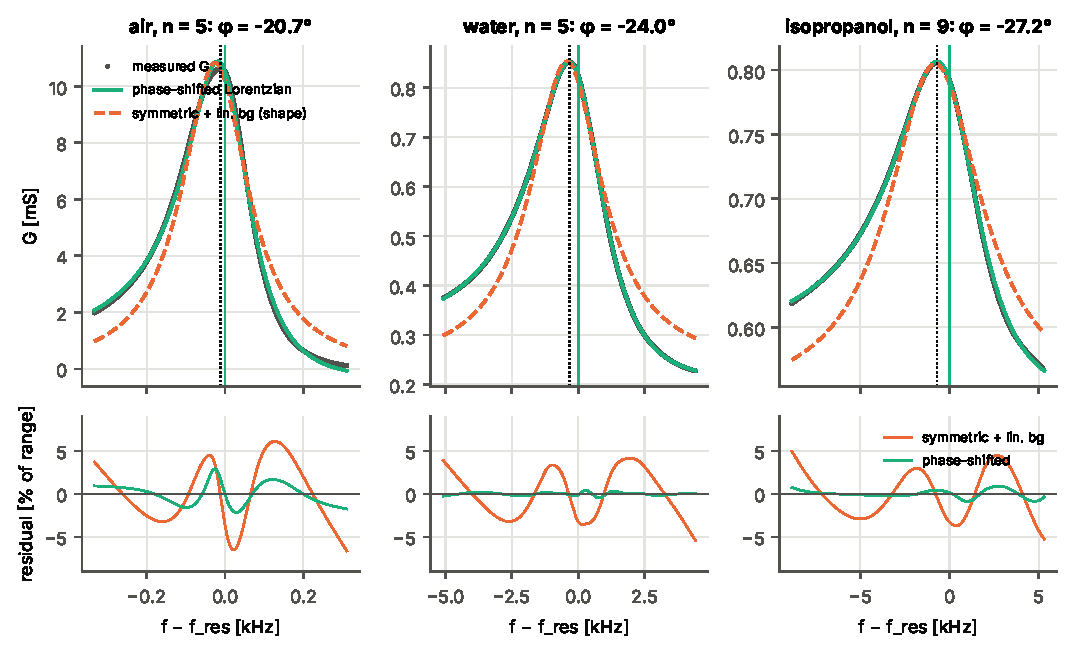
\includegraphics[width=\linewidth]{figures/fig04_fits_residuals.pdf}
\caption{Fig. 4. Conductance (dots) with the phase-shifted Lorentzian
(solid) and the symmetric Lorentzian with linear background (dashed;
drawn without its linear term) on \(\pm3\Gamma_\mathrm{hh}\); below, the
residuals in percent of the range of \(G\). Dotted vertical line:
maximum of \(G\); solid: \(f_\mathrm{res}\) of the phase-shifted fit.}
\end{figure}

\hypertarget{the-bias-of-the-conductance-maximum}{%
\subsection{The bias of the conductance
maximum}\label{the-bias-of-the-conductance-maximum}}

Figure 5 compares the measured offset \(f_{G\max} - f_\mathrm{res}\) on
the 45 sweeps with the prediction of Eq. (8) from the fitted \(\Gamma\)
and \(\varphi\): the difference is +1 ± 28 Hz (sd), at most 77 Hz,
i.e.~0.016 Γ on average and 0.12 Γ at worst; the largest residuals (−40
to −45 Hz) are the liquid fundamentals, where the fold plateau sits
under the peak. The offset is 2--47 Hz in air (0.03--0.25 Γ) and 80--700
Hz in liquid (0.09--0.25 Γ). On the 75 sweeps of the second instrument
(open squares in Fig. 5) the difference is +21 ± 28 Hz, at most 80 Hz
(0.096 Γ), with the same sign pattern: positive on the narrow air peaks,
where the fold plateau sits under the maximum, and within ±0.04 Γ in
liquid. The half-height width is 0.3--8 \% \emph{above} the fitted
\(\Gamma\) in air, as Eq. (9) predicts (0.5--5.5 \%), and 1--8 \%
\emph{below} it in liquid, where the baseline taken on the first 100
samples sits on the skirt of the broadened peak (13--74 \% of the peak
height on \(n \ge 3\)) and raises the half level; the two biases are of
opposite sign and the second dominates in liquid.

\begin{figure}
\centering
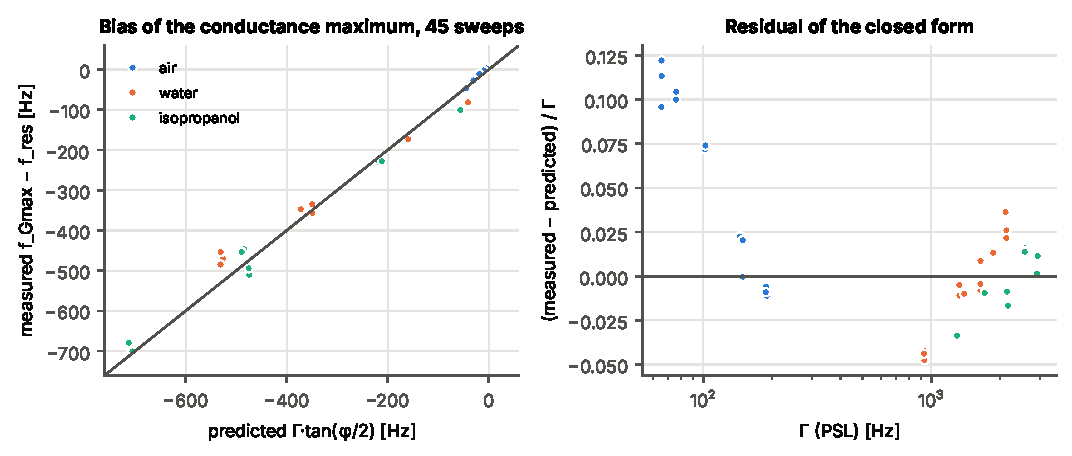
\includegraphics[width=\linewidth]{figures/fig05_argmax_bias.pdf}
\caption{Fig. 5. Left: measured \(f_{G\max} - f_\mathrm{res}\) against
\(\Gamma\tan(\varphi/2)\) from the fit, 45 sweeps of 2026 (filled) and
75 sweeps of the second instrument (open squares); the line is the
identity. Right: residual of the closed form in units of \(\Gamma\).}
\end{figure}

\hypertarget{the-rotation-angle-is-an-instrument-property}{%
\subsection{The rotation angle is an instrument
property}\label{the-rotation-angle-is-an-instrument-property}}

The fitted angle (Fig. 6) is
\(\varphi = -8.0, -14.5, -20.6, -22.9, -26.8^\circ\) on
\(n = 1 \ldots 9\) in air, with a standard deviation over the three
replicas (4--25 min apart) of at most 0.06°. In water and isopropanol it
is \(-5.0, -13.6/-14.3, -24.0/-24.7, -22.5/-21.4, -27.9/-27.2^\circ\):
equal to the air value within 0.2--1.5° on \(n = 3, 7, 9\), 3--4° more
negative on \(n = 5\) and 3° less negative on \(n = 1\). One water sweep
(\(n = 3\), replica 3) gives −17.9° instead of −13.6°; it is the sweep
whose fold decision sits on the threshold (Section 6.9). Five air sweeps
of 2026-09-03 on a 125 MHz board give
\(-7.8, -17.5, -22.6, -25.7, -28.9^\circ\). The angle therefore depends
on the overtone and on the board, not on the load, to within a few
degrees.

Two independent estimates support the interpretation of \(\varphi\) as
the phase of the detector chain. First, the repository's two-channel
forward model, which fits a Butterworth--Van Dyke crystal through the
divider and the detector laws to \(V_\mathrm{MAG}\) and
\(V_\mathrm{PHS}\) jointly with a board phase \(\phi_b\) inside the
modulus of Eq. (6), gives
\(\phi_b = -7.6, -13.8, -19.9, -22.1, -20.4^\circ\) in air: equal to
\(\varphi\) within 0.3--0.8° on \(n = 1\)--7 (crosses in Fig. 6).
Second, the forward model of Section 6.8 returns
\(\varphi_\mathrm{fit} = \phi_b\) to 0.5° when a board phase is imposed
on the transfer function. The angle is not a pure propagation delay: the
short and 50 Ω standards measured on the same front end give a phase
slope of 0.27--0.40° MHz\(^{-1}\) (0.74--1.10 ns), i.e.~1.4--2.0° at 5
MHz and 12--18° at 45 MHz, whereas \(\varphi\) grows roughly as
\(f^{0.55}\) (dotted and dashed lines in Fig. 6).

On the second instrument (2024, Fig. 6, open diamonds) the angle in air
is \(-7.3, -19.7, -19.5, -25.3, -27.9^\circ\) on \(n = 1 \ldots 9\) (sd
over three replicas ≤ 0.13°) and in the four liquids \(+0.7\) to
\(+1.2^\circ\), \(-18.8\) to \(-20.8^\circ\), \(-14.3\) to
\(-14.6^\circ\), \(-27.5\) to \(-28.7^\circ\), \(-30.4\) to
\(-31.9^\circ\) (sd ≤ 0.07°). Three facts follow. The two instruments
agree within 1--3° on \(n = 1, 5, 7, 9\) in air, but differ by 5° on
\(n = 3\), where the second instrument reads \(-19.7^\circ\) against
\(-14.5^\circ\): on that board \(\varphi(3) \approx \varphi(5)\) in air
and \(\varphi(5)\) is \emph{smaller} in magnitude than \(\varphi(3)\) in
liquid, so the angle is not a monotonic function of frequency. The angle
is independent of the glucose concentration within 2° on every overtone,
which confirms it as an instrument property rather than a property of
the load, and its sign on the fundamental in liquid is opposite between
the instruments (\(+1^\circ\) against \(-5^\circ\)), with the first
instrument reading \(-8^\circ\) in air on the same overtone. A
least-squares decomposition into a constant and a delay,
\(\varphi = \varphi_0 - 360^\circ f\tau\), gives
\(\varphi_0 = -8.2^\circ\), \(\tau = 1.31\) ns (rms 2.6°) for the second
instrument in air and \(\varphi_0 = -7.0^\circ\), \(\tau = 1.28\) ns
(rms 1.2°) for board 1920 in air (\(-7.9^\circ\), 1.40 ns on
2026-09-03), i.e.~the same two parameters on both boards within the
scatter; in the liquids of 2024 the fundamental at \(+1^\circ\) pulls
\(\varphi_0\) to 0 to \(-1^\circ\) (rms 4.6--5.4°) and on \(n = 3\)--9
alone \(\varphi_0 = -7.4\) to \(-11.0^\circ\). This decomposition is an
approximation --- the rms is 1--5° and both parameters move when
\(n = 1\) is excluded --- and it is reported to make the comparison
between instruments explicit; the resistive standards of board 1920 had
given only the delays above and intercepts of \(-0.1^\circ\) and
\(-3.5^\circ\), and the \(f^{0.55}\) growth, not a constant offset.

\begin{figure}
\centering
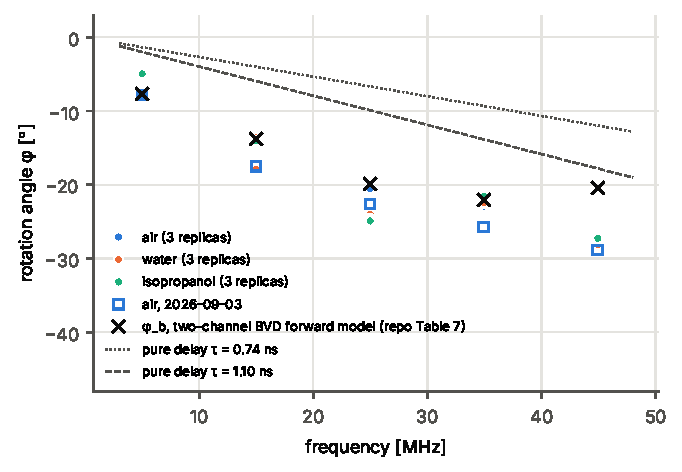
\includegraphics[width=\linewidth]{figures/fig06_phi_vs_frequency.pdf}
\caption{Fig. 6. Rotation angle \(\varphi\) of the phase-shifted
Lorentzian against frequency: three replicas per load on 2026-09-11; air
sweeps of 2026-09-03; the board phase \(\phi_b\) of the repository's
two-channel forward model (crosses); the second instrument of 2024 in
air and in the four liquids (open diamonds); the phase of a pure delay
for the two delays measured on the resistive standards, and the
least-squares lines \(\varphi_0 - 360^\circ f\tau\) for the two
instruments in air.}
\end{figure}

\hypertarget{air-to-liquid-shifts-against-kanazawagordon}{%
\subsection{Air-to-liquid shifts against
Kanazawa--Gordon}\label{air-to-liquid-shifts-against-kanazawagordon}}

Table 1 gives \(f\), \(\Gamma\) and \(D\) per load and overtone for the
two main estimators; Table 2 the shifts and the three error metrics for
all estimators on overtones 3--9; Fig. 7 the shifts against the theory;
Fig. 8 the error metrics per estimator.

\textbf{Table 1.} Resonance frequency, half-bandwidth and dissipation
per load and overtone (mean ± sd of three sweeps): A = maximum of \(G\)
+ half height; P = phase-shifted Lorentzian (\(\varphi\) in degrees).

\begin{longtable}[]{@{}
  >{\raggedright\arraybackslash}p{(\columnwidth - 16\tabcolsep) * \real{0.1111}}
  >{\raggedright\arraybackslash}p{(\columnwidth - 16\tabcolsep) * \real{0.1111}}
  >{\raggedright\arraybackslash}p{(\columnwidth - 16\tabcolsep) * \real{0.1111}}
  >{\raggedright\arraybackslash}p{(\columnwidth - 16\tabcolsep) * \real{0.1111}}
  >{\raggedright\arraybackslash}p{(\columnwidth - 16\tabcolsep) * \real{0.1111}}
  >{\raggedright\arraybackslash}p{(\columnwidth - 16\tabcolsep) * \real{0.1111}}
  >{\raggedright\arraybackslash}p{(\columnwidth - 16\tabcolsep) * \real{0.1111}}
  >{\raggedright\arraybackslash}p{(\columnwidth - 16\tabcolsep) * \real{0.1111}}
  >{\raggedright\arraybackslash}p{(\columnwidth - 16\tabcolsep) * \real{0.1111}}@{}}
\toprule\noalign{}
\begin{minipage}[b]{\linewidth}\raggedright
load
\end{minipage} & \begin{minipage}[b]{\linewidth}\raggedright
n
\end{minipage} & \begin{minipage}[b]{\linewidth}\raggedright
\(f\) (A) {[}Hz{]}
\end{minipage} & \begin{minipage}[b]{\linewidth}\raggedright
\(f\) (P) {[}Hz{]}
\end{minipage} & \begin{minipage}[b]{\linewidth}\raggedright
\(\Gamma\) (A) {[}Hz{]}
\end{minipage} & \begin{minipage}[b]{\linewidth}\raggedright
\(\Gamma\) (P) {[}Hz{]}
\end{minipage} & \begin{minipage}[b]{\linewidth}\raggedright
\(D\) (A) {[}10⁻⁶{]}
\end{minipage} & \begin{minipage}[b]{\linewidth}\raggedright
\(D\) (P) {[}10⁻⁶{]}
\end{minipage} & \begin{minipage}[b]{\linewidth}\raggedright
\(\varphi\) {[}°{]}
\end{minipage} \\
\midrule\noalign{}
\endhead
\bottomrule\noalign{}
\endlastfoot
air & 1 & 5 004 598 ± 2 & 5 004 596 ± 2 & 65.4 ± 0.2 & 65.6 ± 0.1 & 26.1
& 26.2 & −8.0 \\
air & 3 & 14 988 738 ± 8 & 14 988 740 ± 7 & 78.0 ± 0.1 & 76.0 ± 0.1 &
10.4 & 10.1 & −14.5 \\
air & 5 & 24 973 688 ± 13 & 24 973 699 ± 13 & 108.0 ± 0.8 & 102.4 ± 0.7
& 8.6 & 8.2 & −20.6 \\
air & 7 & 34 957 566 ± 22 & 34 957 593 ± 21 & 158.7 ± 2.6 & 147.6 ± 2.3
& 9.1 & 8.4 & −22.9 \\
air & 9 & 44 943 110 ± 23 & 44 943 157 ± 23 & 203.7 ± 0.8 & 188.7 ± 1.0
& 9.1 & 8.4 & −26.8 \\
water & 1 & 5 003 826 ± 3 & 5 003 909 ± 2 & 937 ± 3 & 934 ± 4 & 374.5 &
373.5 & −5.0 \\
water & 3 & 14 987 288 ± 52 & 14 987 478 ± 16 & 1318 ± 33 & 1351 ± 38 &
175.9 & 180.3 & −15.0 \\
water & 5 & 24 971 737 ± 24 & 24 972 088 ± 13 & 1582 ± 2 & 1646 ± 1 &
126.7 & 131.8 & −24.0 \\
water & 7 & 34 955 379 ± 19 & 34 955 726 ± 18 & 1823 ± 3 & 1872 ± 3 &
104.3 & 107.1 & −22.5 \\
water & 9 & 44 940 695 ± 37 & 44 941 165 ± 29 & 2100 ± 1 & 2130 ± 10 &
93.4 & 94.8 & −27.9 \\
isopropanol & 1 & 5 003 555 ± 2 & 5 003 656 ± 2 & 1286 ± 1 & 1297 ± 1 &
513.9 & 518.4 & −5.0 \\
isopropanol & 3 & 14 986 825 ± 3 & 14 987 054 ± 5 & 1670 ± 1 & 1719 ± 1
& 222.9 & 229.3 & −14.3 \\
isopropanol & 5 & 24 971 122 ± 10 & 24 971 627 ± 1 & 2025 ± 4 & 2167 ±
13 & 162.2 & 173.5 & −24.7 \\
isopropanol & 7 & 34 954 645 ± 5 & 34 955 093 ± 0.3 & 2383 ± 2 & 2570 ±
2 & 136.4 & 147.0 & −21.4 \\
isopropanol & 9 & 44 939 783 ± 1 & 44 940 476 ± 12 & 2710 ± 3 & 2925 ±
12 & 120.6 & 130.2 & −27.2 \\
\end{longtable}

\textbf{Table 2.} Air-to-liquid shifts on overtones 3--9 against
Kanazawa--Gordon at 25 °C, range over \(n\) and both liquids.
\(\epsilon_f = \Delta f/\Delta f_\mathrm{KG} - 1\);
\(\epsilon_\Gamma = \Delta\Gamma/\Delta\Gamma_\mathrm{KG} - 1\);
\(\rho_N = |\Delta f|/\Delta\Gamma\). The magnitude estimator's ``Γ'' is
half its −3 dB width, undefined on \(n \ge 5\) in liquid.

\begin{longtable}[]{@{}
  >{\raggedright\arraybackslash}p{(\columnwidth - 10\tabcolsep) * \real{0.1667}}
  >{\raggedright\arraybackslash}p{(\columnwidth - 10\tabcolsep) * \real{0.1667}}
  >{\raggedright\arraybackslash}p{(\columnwidth - 10\tabcolsep) * \real{0.1667}}
  >{\raggedright\arraybackslash}p{(\columnwidth - 10\tabcolsep) * \real{0.1667}}
  >{\raggedright\arraybackslash}p{(\columnwidth - 10\tabcolsep) * \real{0.1667}}
  >{\raggedright\arraybackslash}p{(\columnwidth - 10\tabcolsep) * \real{0.1667}}@{}}
\toprule\noalign{}
\begin{minipage}[b]{\linewidth}\raggedright
estimator
\end{minipage} & \begin{minipage}[b]{\linewidth}\raggedright
\(\epsilon_f\) {[}\%{]}
\end{minipage} & \begin{minipage}[b]{\linewidth}\raggedright
\(\epsilon_\Gamma\) {[}\%{]}
\end{minipage} & \begin{minipage}[b]{\linewidth}\raggedright
\(\rho_N\)
\end{minipage} & \begin{minipage}[b]{\linewidth}\raggedright
\(\max|\epsilon_f|\) {[}\%{]}
\end{minipage} & \begin{minipage}[b]{\linewidth}\raggedright
\(\max|\epsilon_\Gamma|\) {[}\%{]}
\end{minipage} \\
\midrule\noalign{}
\endhead
\bottomrule\noalign{}
\endlastfoot
(M) magnitude maximum & +52 \ldots{} +92 & +40 \ldots{} +309 & 0.42
\ldots{} 1.08 & 92 & 309 \\
(A) max of \(G\) + half height & +19.5 \ldots{} +29.5 & −7.4 \ldots{}
+6.3 & 1.17 \ldots{} 1.34 & 29.5 & 7.4 \\
(MP) half-height midpoint & +33 \ldots{} +47 & −7.4 \ldots{} +6.3 & 1.27
\ldots{} 1.53 & 47 & 7.4 \\
(S) symmetric, constant bg & +33 \ldots{} +52 & +8 \ldots{} +30 & 1.15
\ldots{} 1.34 & 52 & 30 \\
(S) symmetric, linear bg & +24.5 \ldots{} +34.4 & −3.0 \ldots{} +11.3 &
1.14 \ldots{} 1.33 & 34 & 11 \\
(C) BVD circle (repository) & −2.5 \ldots{} +37.9 & −9.6 \ldots{} +25.7
& 1.01 \ldots{} 1.14 & 38 & 26 \\
(P) phase-shifted Lorentzian & −1.4 \ldots{} +8.2 & −3.9 \ldots{} +9.3 &
0.98 \ldots{} 1.08 & 8.2 & 9.3 \\
\end{longtable}

\begin{figure}
\centering
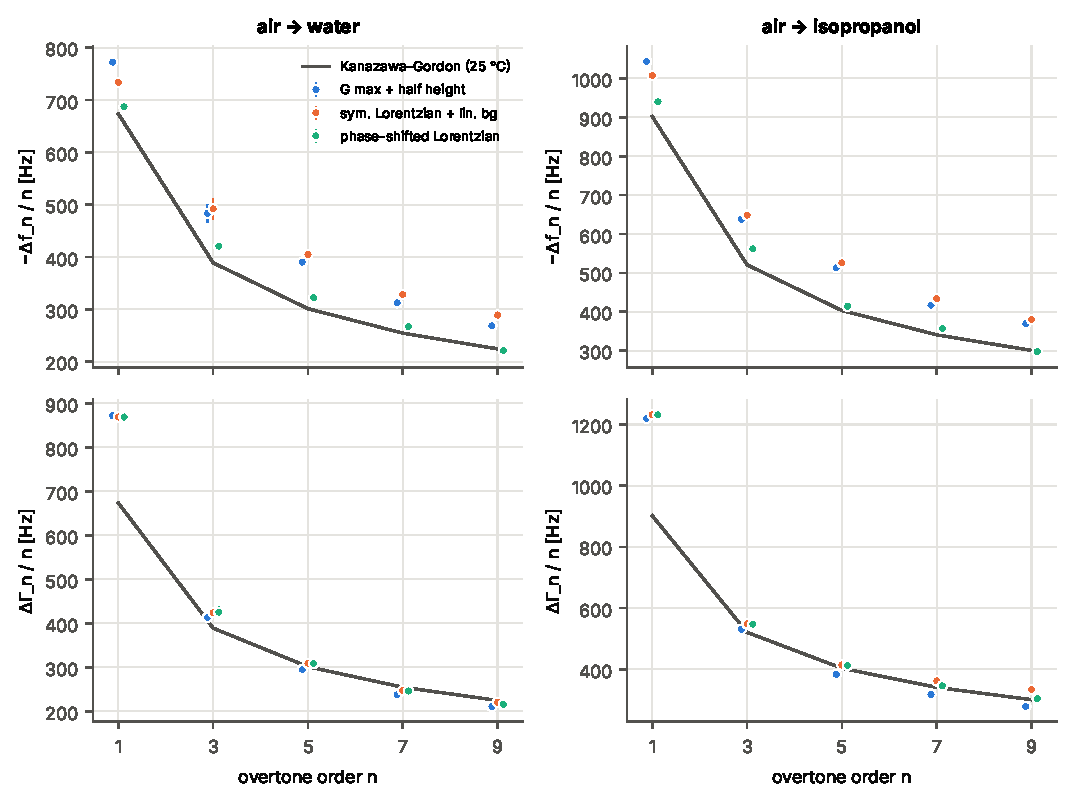
\includegraphics[width=\linewidth]{figures/fig07_shifts_vs_KG.pdf}
\caption{Fig. 7. Overtone-normalised shifts \(-\Delta f_n/n\) (top) and
\(\Delta\Gamma_n/n\) (bottom) against the overtone order for the maximum
of \(G\), the symmetric Lorentzian with linear background and the
phase-shifted Lorentzian, with the Kanazawa--Gordon prediction at 25 °C.
Error bars (mostly within the markers) are the replica scatter divided
by \(n\).}
\end{figure}

Per overtone, the phase-shifted Lorentzian gives \(\epsilon_f\) = +8.2,
+7.0, +4.8, −1.4 \% (water, \(n\) = 3, 5, 7, 9) and +7.9, +2.7, +4.8,
−1.0 \% (isopropanol), \(\epsilon_\Gamma\) = +9.3, +2.5, −3.3, −3.9 \%
(water) and +5.1, +2.3, +1.5, +1.1 \% (isopropanol), and \(\rho_N\) =
0.99, 1.04, 1.08, 1.03 (water) and 1.03, 1.00, 1.03, 0.98 (isopropanol).
The maximum of \(G\) gives \(\epsilon_f\) = +24, +30, +23, +20 \%
(water) and +23, +27, +22, +23 \% (isopropanol) with \(\rho_N\) =
1.17--1.34, and \(\epsilon_\Gamma\) = +6.3, −2.1, −6.6, −6.2 \% (water)
and +1.9, −5.0, −6.8, −7.4 \% (isopropanol). The slopes of a line
through the origin against \(\sqrt n\) (\(n\) = 1--9) are 696 Hz
(\(-\Delta f\)) and 677 Hz (\(\Delta\Gamma\)) in water against 674 Hz
predicted, and 926 and 932 Hz in isopropanol against 902 Hz, with the
phase-shifted fit; 827/656 Hz and 1112/867 Hz with the maximum of \(G\).
The \(\sqrt n\) law itself holds for every estimator (the five points
lie on a line through the origin in both cases); what changes between
estimators is the slope of the frequency line.

\begin{figure}
\centering
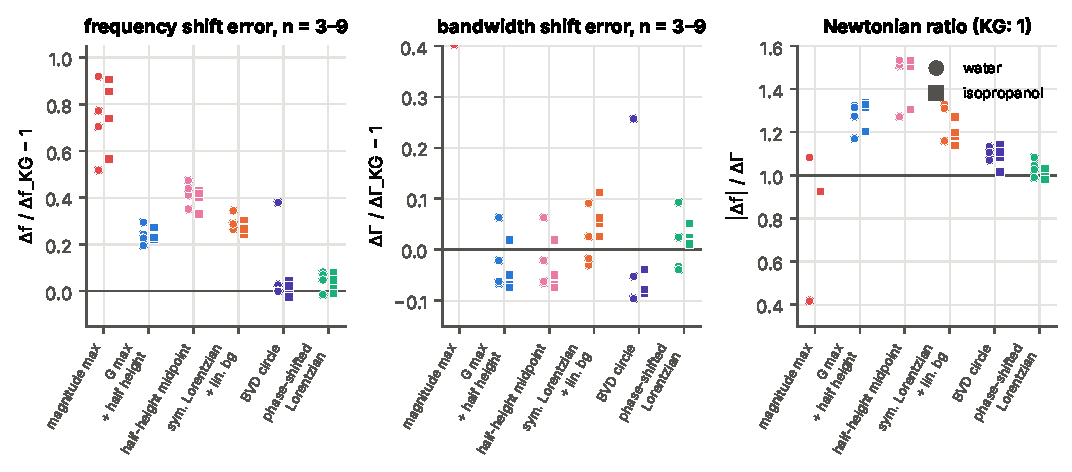
\includegraphics[width=\linewidth]{figures/fig08_estimator_errors.pdf}
\caption{Fig. 8. The three error metrics on overtones 3--9 (circles
water, squares isopropanol) for six estimators.}
\end{figure}

On the second instrument and crystal the ranking repeats, on four
liquids (Table 3, Fig. 12, Fig. 13). Against air, the Newtonian ratio on
overtones 3--9 is 1.20--1.41 with the maximum of \(G\) and 1.01--1.16
with the phase-shifted Lorentzian in water and in the three glucose
solutions alike (the midpoint gives 1.31--1.68, the symmetric Lorentzian
with linear background 1.17--1.47, the circle 0.90--1.16). For water
against Kanazawa--Gordon, \(\Delta f/\Delta f_\mathrm{KG}\) is
1.20--1.36 with the maximum of \(G\) and 1.06--1.13 with the fit, while
\(\Delta\Gamma/\Delta\Gamma_\mathrm{KG}\) is 0.96--1.00 and 0.96--1.05
respectively: as on board 1920, the fit changes the frequency and leaves
the bandwidth. The residual pattern over the overtones is not random:
with the fit the Newtonian ratio is 1.15, 1.01, 1.16, 1.12 on
\(n = 3, 5, 7, 9\) in water and the same to ±0.02 in the three glucose
solutions, i.e.~a zig-zag that is identical in four liquids and
therefore instrumental; it coincides with the anomaly of \(\varphi\) on
the same board (\(|\varphi|\) smallest on \(n = 5\), where the ratio is
closest to one), which suggests that the residual error after the
rotation correction tracks what the single-angle model does not capture
of this board's phase response. The residual frequency excess of water
(+6 to +13 \%) is in the range of the first instrument's (+2 to +8 \%)
within the unmeasured liquid temperature.

\textbf{Table 3.} Second instrument (2024-05-29): air-to-liquid shifts
on overtones 3--9, range over \(n\). Water against Kanazawa--Gordon at
25 °C; the Newtonian ratio for all four liquids. A = maximum of \(G\) +
half height; P = phase-shifted Lorentzian.

\begin{longtable}[]{@{}
  >{\raggedright\arraybackslash}p{(\columnwidth - 4\tabcolsep) * \real{0.3333}}
  >{\raggedright\arraybackslash}p{(\columnwidth - 4\tabcolsep) * \real{0.3333}}
  >{\raggedright\arraybackslash}p{(\columnwidth - 4\tabcolsep) * \real{0.3333}}@{}}
\toprule\noalign{}
\begin{minipage}[b]{\linewidth}\raggedright
quantity
\end{minipage} & \begin{minipage}[b]{\linewidth}\raggedright
A
\end{minipage} & \begin{minipage}[b]{\linewidth}\raggedright
P
\end{minipage} \\
\midrule\noalign{}
\endhead
\bottomrule\noalign{}
\endlastfoot
water, \(\Delta f/\Delta f_\mathrm{KG}\) & 1.20 \ldots{} 1.36 & 1.06
\ldots{} 1.13 \\
water, \(\Delta\Gamma/\Delta\Gamma_\mathrm{KG}\) & 0.96 \ldots{} 1.00 &
0.96 \ldots{} 1.05 \\
\(\rho_N = |\Delta f|/\Delta\Gamma\), water & 1.20 \ldots{} 1.41 & 1.01
\ldots{} 1.16 \\
\(\rho_N\), glucose 5 / 7.5 / 10 \% & 1.21 \ldots{} 1.40 & 1.02 \ldots{}
1.14 \\
fundamental: \(\Delta\Gamma_1/\Delta\Gamma_\mathrm{KG}\), \(\rho_N\)
(water) & 1.04, 1.04 & 1.07, 1.01 \\
\end{longtable}

\begin{figure}
\centering
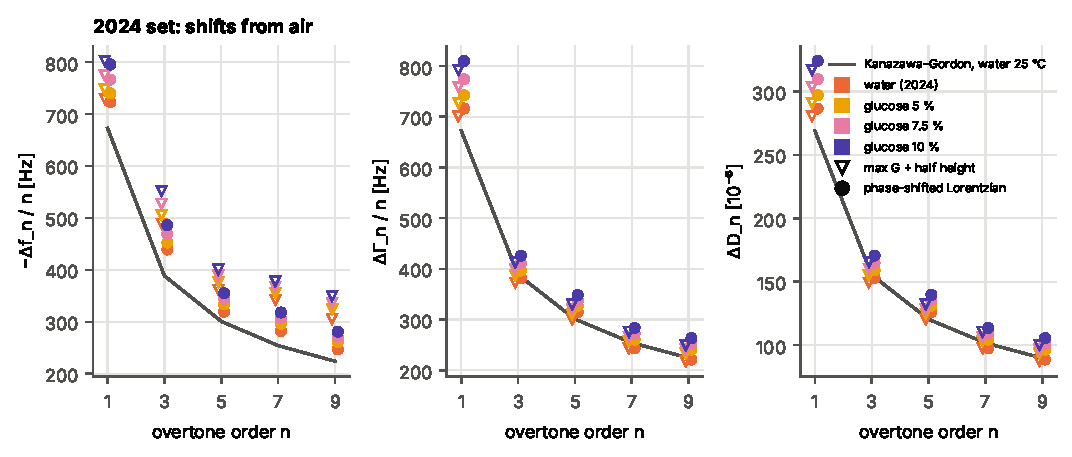
\includegraphics[width=\linewidth]{figures/fig12_glucose_shifts_vs_n.pdf}
\caption{Fig. 12. Second instrument: overtone-normalised shifts from
air, \(-\Delta f_n/n\), \(\Delta\Gamma_n/n\) and \(\Delta D_n\), for
water and the three glucose solutions, with the maximum of \(G\) (open
triangles) and the phase-shifted Lorentzian (filled circles) and the
Kanazawa--Gordon prediction for water.}
\end{figure}

\begin{figure}
\centering
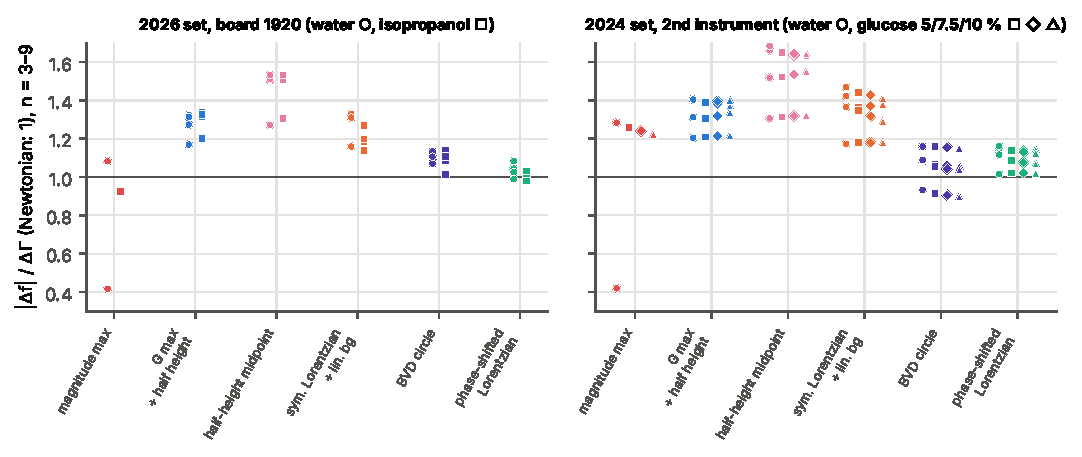
\includegraphics[width=\linewidth]{figures/fig13_newtonian_ratio_two_instruments.pdf}
\caption{Fig. 13. The Newtonian ratio on overtones 3--9 per estimator on
the two instruments: board 1920 (water, isopropanol) and the instrument
of 2024 (water and glucose 5, 7.5, 10 \% w/v).}
\end{figure}

\hypertarget{concentration-series}{%
\subsection{Concentration series}\label{concentration-series}}

Relative to water, the glucose solutions shift the fitted resonance by
\(-17\) to \(-72\) Hz (fundamental) and \(-128\) to \(-307\) Hz (9th
overtone) at 10 \% w/v and broaden it by \(+94\) to \(+379\) Hz (Fig.
14). A straight line through the four concentrations (0, 5, 7.5, 10 \%
w/v) has slopes of \(-7.1, -13.8, -17.8, -24.7, -30.4\) Hz per \% w/v in
\(\Delta f_n\), \(+9.2, +13.1, +16.6, +28.0, +37.8\) Hz per \% w/v in
\(\Delta\Gamma_n\) and \(3.68, 1.75, 1.33, 1.60, 1.68 \times 10^{-6}\)
per \% w/v in \(\Delta D_n\) for \(n = 1 \ldots 9\) (phase-shifted
Lorentzian, ordinary least squares with intercept); the maximum of \(G\)
gives the same bandwidth slopes within 1 Hz per \% and frequency slopes
1--30 \% steeper on \(n \ge 3\), because its bias grows with the width.
On \(n = 1\) and 3 the 5 \% point lies 12--18 Hz below the line (\(R^2\)
= 0.91 and 0.94, against 0.986--0.990 on \(n \ge 5\)); the replica
scatter there is 0.3--3 Hz, so the departure is systematic, and it is of
the size of the 10--20 Hz drift of the air baseline during an hour on
the first instrument, which this experiment, with no return to water
between concentrations, cannot separate from a real non-linearity. The
square of the air-referenced frequency shift relative to water,
\((\Delta f/\Delta f_\mathrm{water})^2 = \rho\eta/(\rho\eta)_\mathrm{water}\)
for a Newtonian liquid, averaged over \(n = 3\)--9, is 1.094, 1.171 and
1.256 at 5, 7.5 and 10 \% w/v with the phase-shifted Lorentzian and
1.089, 1.171 and 1.257 with the maximum of \(G\): the two estimators
agree on the ratio to 0.5 \% although they disagree on each shift by
20--30 \%, because the rotation bias is a nearly constant fraction of
the shift at a given overtone and cancels in the quotient. The same
ratio from the bandwidth is 1.08--1.18, 1.15--1.30 and 1.22--1.42,
growing with the overtone faster than the frequency-based one, a
difference the Newtonian model does not predict and that the data of one
day on one instrument, with the liquid temperature unmeasured, cannot
resolve. No tabulated density or viscosity of the glucose solutions is
used here.

\begin{figure}
\centering
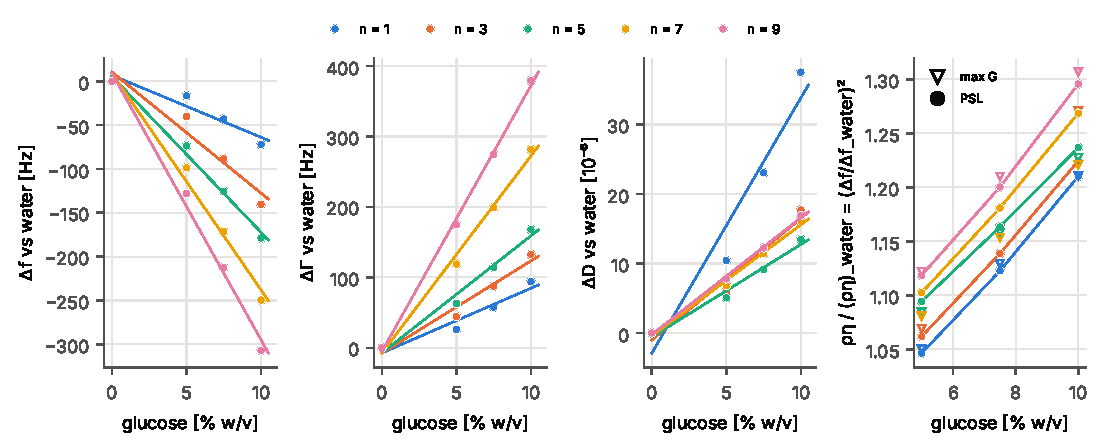
\includegraphics[width=\linewidth]{figures/fig14_glucose_concentration.pdf}
\caption{Fig. 14. Second instrument: shifts relative to water of the
fitted resonance frequency, half-bandwidth and dissipation against
glucose concentration, one line per overtone (ordinary least squares
with intercept), and the ratio \(\rho\eta/(\rho\eta)_\mathrm{water}\)
from the air-referenced frequency shifts with the two estimators.}
\end{figure}

\hypertarget{what-reconstruction-buys-and-what-the-rotation-buys}{%
\subsection{What reconstruction buys and what the rotation
buys}\label{what-reconstruction-buys-and-what-the-rotation-buys}}

Table 2 separates the two steps. Going from the magnitude channel to the
reconstructed conductance (M → A) removes two thirds of the frequency
error (+52\ldots+92 \% → +20\ldots+30 \%) and, more importantly,
produces a bandwidth with a physical definition: the magnitude curve's
−3 dB width is undefined inside the sweep window for \(n \ge 5\) in
liquid and its −0.3 dB width (the production software's ``dissipation'')
grows to 3.7--6.4 kHz at \(n\) = 9, ten times the theory's
\(\Delta\Gamma\), with no counterpart in it (Section 6.10). The
half-height width of \(G\) is within ±7.4 \% of Kanazawa--Gordon on
overtones 3--9. Going from the maximum of \(G\) to the phase-shifted fit
(A → P) removes the remaining +20\ldots+30 \% on frequency, which Eq.
(8) attributes to the rotation, and leaves the bandwidth essentially
unchanged (−3.9\ldots+9.3 \%, the +9.3 \% being the two-state water
sweep of Section 6.9; the fitted \(\Gamma\) is 2--8 \% above the
half-height width in liquid, which corrects the baseline bias of Section
6.3). The improvement produced by the rotated Lorentzian is therefore a
\emph{frequency} improvement; the bandwidth was already right after
reconstruction, and the symmetric Lorentzian --- which models the shape
but not the rotation --- improves neither (its \(\epsilon_f\) is
+24\ldots+34 \%, worse than the maximum of \(G\), as the ≈1.25
\(\Gamma\tan(\varphi/2)\) bias of Section 4.2 predicts).

\hypertarget{forward-model-when-is-the-rotated-lorentzian-the-right-model}{%
\subsection{Forward model: when is the rotated Lorentzian the right
model?}\label{forward-model-when-is-the-rotated-lorentzian-the-right-model}}

A board phase does not multiply the admittance; it multiplies the
\emph{measured transfer function}, \(H_\mathrm{meas} = He^{j\phi_b}\).
Inverting exactly with that phase gives
\(Y' = 1/[(Z_q + R_{17})e^{-j\phi_b} - R_{17}]\), a Möbius
transformation of \(Y_q\) that reduces to the rotation
\(Y_q e^{j\phi_b}\) only when \(|Z_q| \gg R_{17}\). We therefore built a
Butterworth--Van Dyke crystal of known \(f_s\), \(\Gamma\), \(R_1\) and
\(C_0\), sent it through the divider and the detector laws with a board
phase on \(\angle H\), an offset \(\delta\), the fold, the ADC
quantisation and the firmware carry-over, and ran the same chain and
estimators (Fig. 10, Supplementary \texttt{forward\_model.md}).
Findings: (i) the fitted angle equals the imposed board phase to 0.5° on
every case; (ii) with \(\phi_b = 0\) both estimators recover \(f_s\) to
the grid; (iii) with \(\phi_b = -8\) to \(-25^\circ\) the maximum of
\(G\) is off by \(-91\) to \(-743\) Hz on liquid-like cases, the
phase-shifted fit by \(-7\) to \(-59\) Hz (≤2 \% of Γ), the symmetric
fit by \(-96\) to \(-833\) Hz; (iv) the residual error of the
phase-shifted fit scales as \(\approx -0.34\,\Gamma\,(R_{17}/R_1)\) at
\(\phi_b = -20^\circ\): \(-344\) Hz at \(R_1 = R_{17}\) and \(-12\) Hz
at \(R_1 = 1.6\) kΩ for Γ = 1 kHz, so for the air-like cases (Γ =
65--190 Hz, \(R_1\) = 36--204 Ω) it is \(-12\) to \(-39\) Hz, one third
to one half of the argmax bias there; (v) when a fold exists, the offset
\(\delta\) is removed and does not move \(f_\mathrm{res}\) or \(\Gamma\)
(≤0.5 Hz for \(\delta\) = −3\ldots+7°), but the smoothing rounds the
vertex and the recovered \(\delta\) is 1.0--2.3° more negative than the
true one; (vi) when there is no fold, an uncorrectable \(\delta\) of ±5°
enters the fitted angle almost one to one
(\(\varphi_\mathrm{fit} \approx \phi_b - \delta\)) and moves
\(f_\mathrm{res}\) by ≤10 Hz and \(\Gamma\) by ≤7 Hz; (vii) a ±5 \%
error on the magnitude slope (±3 to ±15 \% on \(M\)) moves
\(f_\mathrm{res}\) by ≤15 Hz and \(\Gamma\) by ≤1 \%, but
\(R_m = 1/G_\mathrm{max}\) by 10--40 \%, and even with an ideal
magnitude channel \(R_m\) is 24--39 \% low in liquid because the peak
height is reduced by \(\cos^2(\varphi/2)\) and by the baseline; (viii)
the firmware carry-over moves \(f_\mathrm{res}\) by ≤2 Hz. The
instrument's smoothing (Savitzky--Golay 51 points plus spline) widens a
65 Hz half-bandwidth by 6.6 Hz (+10 \%) and a 190 Hz one by 3.5 Hz; it
is negligible in liquid.

\begin{figure}
\centering
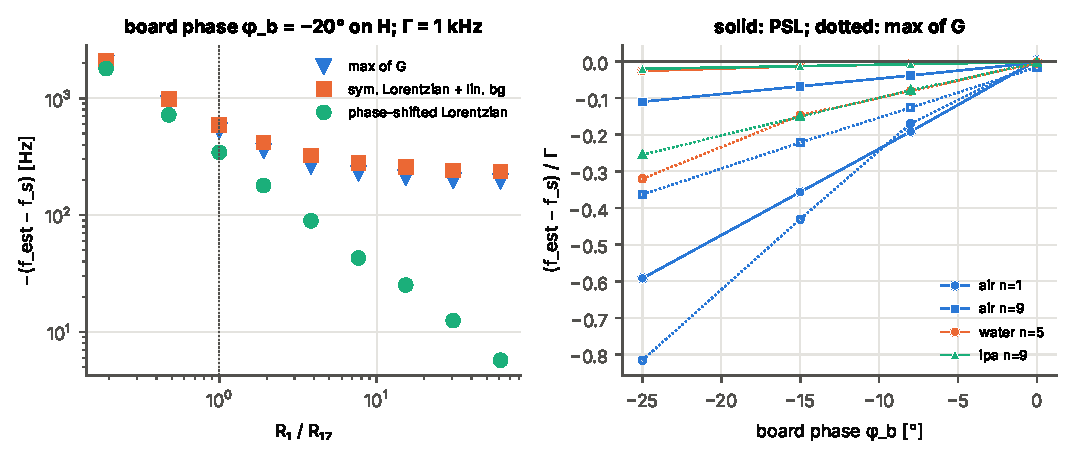
\includegraphics[width=\linewidth]{figures/fig10_forward_model.pdf}
\caption{Fig. 10. Forward model. Left: error of three estimators against
\(R_1/R_{17}\) for a board phase of −20° on the transfer function (Γ = 1
kHz). Right: error in units of Γ against the board phase for four
measured-like cases; solid: phase-shifted fit; dotted: maximum of
\(G\).}
\end{figure}

\hypertarget{repeatability-failure-modes-and-the-firmware-correction}{%
\subsection{Repeatability, failure modes and the firmware
correction}\label{repeatability-failure-modes-and-the-firmware-correction}}

Over the three sweeps of each plateau the standard deviation of
\(f_\mathrm{res}\) is 1.5--23 Hz in air (growing with \(n\) because the
air baseline was still drifting at −0.3 to −2 Hz/min) and 0.3--29 Hz in
liquid for both estimators, and that of \(\Gamma\) is ≤2.6 Hz in air and
≤13 Hz in liquid (Fig. 9). The phase-shifted fit is at least as
repeatable as the maximum of \(G\) and better on \(n \ge 5\) in
isopropanol (0.3--12 Hz against 0.6--10 Hz on \(f\)). On the second
instrument the three replicas, taken 3--10 min apart on a quieter
baseline, scatter by ≤3 Hz in air and ≤8 Hz in liquid for the fit, and
≤36 Hz for the maximum of \(G\) (water, \(n\) = 9, a flat peak on a 1 Hz
grid); all 75 fits converged and passed the gate. The fit's covariance
gives 0.1--0.8 Hz on \(f_\mathrm{res}\), an order of magnitude below the
replica scatter, because the residual is structured; the replica scatter
is the number to quote. One sweep is anomalous: water, \(n\) = 3,
replica 3, whose phase peak grazes zero (fold depth 0.880 against a
threshold of 0.88); the instrument's datalog shows the logged pair
alternating between two states 105 Hz apart from 13:12 onwards, the
fitted \(\varphi\) is 4.3° off its replicas, and the 0.2 \% firmware
correction flips its fold decision and moves its \(f_\mathrm{res}\) by
37 Hz (phase-shifted) and 111 Hz (maximum of \(G\)). On the other 44
sweeps the correction changes \(f_\mathrm{res}\) by ≤2.2 Hz and
\(\Gamma\) by ≤1.7 Hz. The repository's BVD circle estimator returns a
scatter of 309 Hz on that overtone, because the sign of \(B\) depends on
the same decision; the conductance-only estimators do not use \(B\) and
carry only the 50 Hz state change.

\begin{figure}
\centering
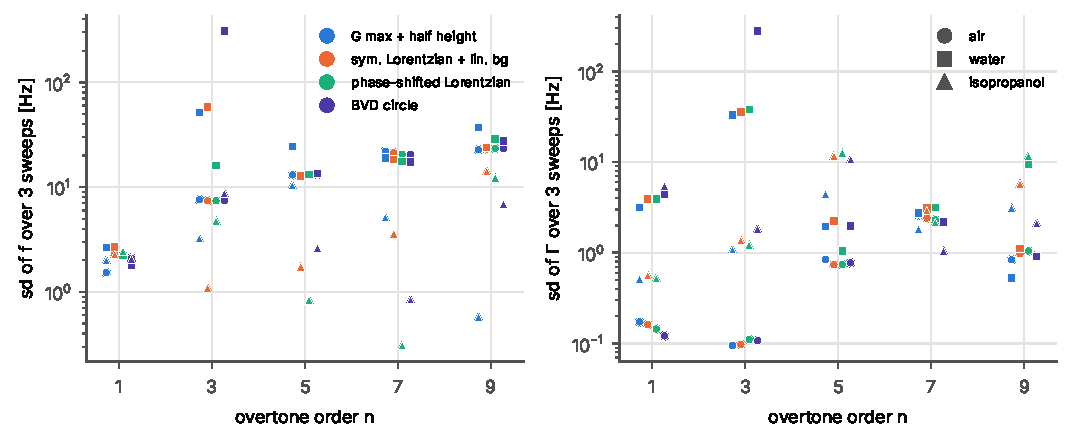
\includegraphics[width=\linewidth]{figures/fig09_repeatability.pdf}
\caption{Fig. 9. Standard deviation over the three plateau sweeps of
\(f_\mathrm{res}\) (left) and \(\Gamma\) (right) per estimator, overtone
and load.}
\end{figure}

\hypertarget{the-production-estimator-on-the-same-acquisitions}{%
\subsection{The production estimator on the same
acquisitions}\label{the-production-estimator-on-the-same-acquisitions}}

The instrument logged, at the same instants, the production magnitude
estimator (maximum of the baseline-corrected magnitude in dB and its
full width 0.3 dB below the maximum) and the conductance estimator (Fig.
11, Supplementary \texttt{datalogs.md}). On the last 10 min of each
plateau of 2026-09-11 (duplicate rows written in bursts, 95 of 486,
removed) the magnitude maximum gives \(\epsilon_f\) = +51, +69, +76, +89
\% (water, \(n\) = 3--9) and +57, +74, +85, +90 \% (isopropanol),
against +23, +29, +22, +18 \% and +22, +27, +22, +22 \% for the maximum
of \(G\) logged live; the run of 2026-09-10 (2.5 min plateaus) gives
+51\ldots+98 \% and +22\ldots+30 \%. The −0.3 dB width changes by
0.77--3.7 kHz (water) and 1.1--6.4 kHz (isopropanol) on \(n\) = 3--9,
where the theory's \(\Delta\Gamma\) is 1.2--2.7 kHz; in air it is 63--70
Hz at the fundamental against \(\Gamma\) = 49--65 Hz. The live
conductance estimator reproduces the offline analysis of the same sweeps
within the plateau drift.

\begin{figure}
\centering
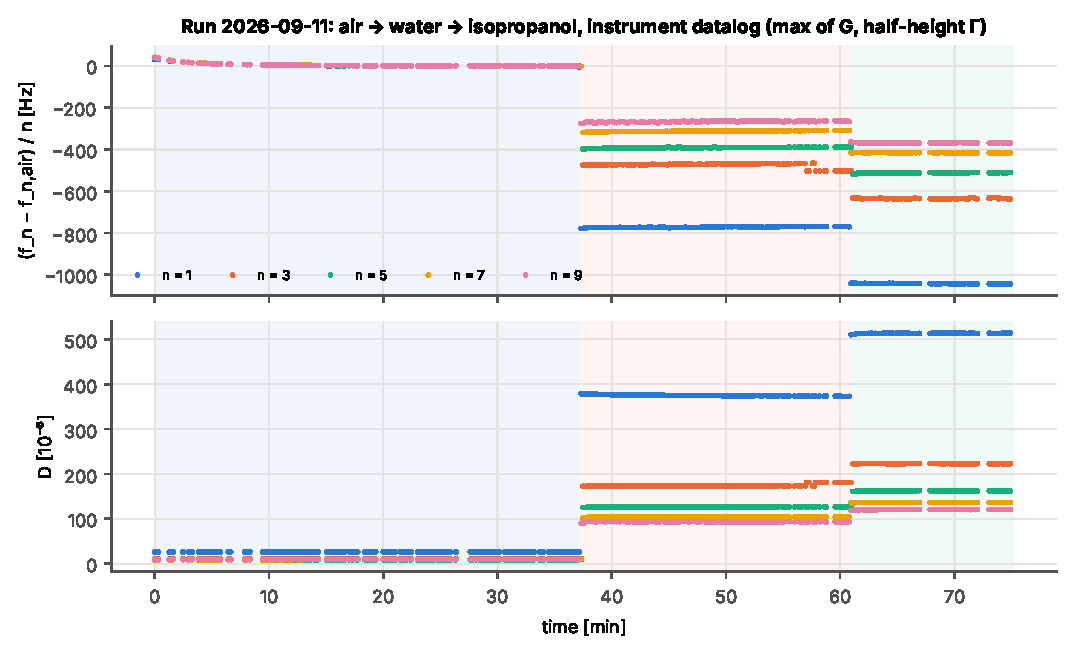
\includegraphics[width=\linewidth]{figures/fig11_datalog_run.pdf}
\caption{Fig. 11. The run of 2026-09-11 as logged by the instrument
(maximum of \(G\), half-height \(\Gamma\)): overtone-normalised
frequency relative to the air value and dissipation factor against time;
shaded: air, water, isopropanol.}
\end{figure}

\hypertarget{the-fundamental}{%
\subsection{The fundamental}\label{the-fundamental}}

The fundamental does not follow the theory with any estimator:
\(\epsilon_\Gamma\) = +29 \% (water) and +35--37 \% (isopropanol),
\(\rho_N\) = 0.76--0.89, while \(\epsilon_f\) is +2 to +4 \% with the
phase-shifted fit. Its dissipation in air is 26 × 10⁻⁶ (2026-09-11) and
19.6 × 10⁻⁶ (2026-09-10) against 8--10 and 5--6 × 10⁻⁶ on the overtones,
and the smoothing bias of Section 6.8 accounts for only a tenth of the
air value. The excess is in the bandwidth and is present before the
liquid is added: we attribute it to the sensor and its mounting rather
than to the method (Section 7). The second instrument and crystal do not
show it: there \(\Delta\Gamma_1/\Delta\Gamma_\mathrm{KG}\) = 1.04
(maximum of \(G\)) and 1.07 (fit) and the Newtonian ratio on the
fundamental is 1.04 and 1.01, while the air dissipation of that
crystal's fundamental is even higher (44--46 × 10⁻⁶, \(\Gamma\) =
110--115 Hz). The fundamental excess of 2026 therefore follows the first
sensor or board, not the method and not the air damping as such; the
two-board, two-sensor cross test of the remaining experiments is what
separates sensor from board.

\hypertarget{discussion}{%
\section{Discussion}\label{discussion}}

\textbf{Physical response, instrumental rotation, detector limits.} The
data separate into three layers. The physical QCM response --- the
\(\sqrt n\) scaling of both shifts, their equality for a Newtonian
liquid, their magnitude for water and isopropanol --- is recovered on
overtones 3--9 to within +8 \% in frequency and ±9 \% in bandwidth once
the resonance is read with the phase-shifted Lorentzian, and the
Newtonian ratio, which is independent of the liquid constants, is
0.98--1.08. The instrumental rotation \(\varphi\) is reproducible to
0.1--0.3°, equal in air and in liquid to a few degrees, equal to the
board phase of an independent two-channel model, and it is the whole of
the 20--30 \% frequency excess of the conductance maximum, as Eq. (8)
predicts to +1 ± 28 Hz on 45 sweeps. Its frequency dependence
(\(f^{0.55}\), not linear) rules out a pure cable delay as the only
cause; the AD8302's own phase response (non-linear within
\textasciitilde18° of 0° and 180°), the drive network and the input
matching are candidates that only a calibration with reference loads in
the operating range will separate. The detector's limits are visible in
the residuals: the fold is rounded over 20--50 Hz in air (the detector
compresses the last degrees towards 0°), the divider ratio in liquid
sits at the edge of the specified range and the locus is 5--18 \% out of
round there, and the one unstable sweep is the one whose phase peak
grazes zero.

\textbf{Correction and model assumptions.} The rotated Lorentzian
assumes that the error is a multiplication of the admittance by a
complex constant. The forward model shows that for a phase error on the
transfer function this is exact only when \(|Z_q| \gg R_{17}\); in
liquid (\(R_m/R_{17}\) = 12--24) the residual is ≤2 \% of Γ, i.e.~≤60
Hz, and in air (\(R_m/R_{17}\) = 0.7--4) the correction removes only
half to two thirds of the argmax bias --- which in air is 2--47 Hz and
matters little for shifts of hundreds of hertz, but matters if absolute
air values are compared between instruments. The residual +2 to +8 \%
frequency excess of the phase-shifted fit on \(n\) = 3--7 is of the size
of the sum of the Möbius residual, the ±2--3 \% uncertainty from the
unmeasured liquid temperature and the clipping of the ±3Γ window by the
sweep on the right side for \(n \ge 5\) in isopropanol (2.2--3.0 Γ
available); the data do not separate these.

\textbf{Robustness.} The result does not depend on the smoothing
(\(f_\mathrm{res}\) within 5 Hz, \(\Gamma\) within 29 Hz between raw and
smoothed data, repository block A2), on the phase offset (±5° → ≤21 Hz),
on the fit window (±2 to ±6 Γ → ≤60 Hz) or on the 0.2 \% firmware bias
(≤2 Hz), with the single exception of the sweep whose fold decision sits
on the threshold. The acceptance gate never fired on 45 sweeps; its
parameters were set at ten times the observed spread and are
instrument-specific.

\textbf{A second instrument.} The 2024 set tests the method where it was
not tuned: another board, another crystal, the production software of
the time, four liquids. The ranking of the estimators and the size of
the correction repeat (Newtonian ratio 1.20--1.41 → 1.01--1.16; water
frequency shift +20\ldots+36 \% → +6\ldots+13 \%), the bandwidth is
again right before the fit, and the closed form of the bias holds (+21 ±
28 Hz on 75 sweeps). Two things do not repeat: the rotation angle
differs by 5° on the 3rd overtone and is not monotonic in frequency on
that board, so \(\varphi(n)\) must be measured per instrument and cannot
be written as a universal function; and the fundamental follows the
theory there, which places the +29\ldots+37 \% excess of 2026 on the
first sensor or board. The residual zig-zag over the overtones,
identical in four liquids, says that a single angle per overtone leaves
a few percent of instrument response uncorrected, consistent with the
Möbius residual and with whatever in the board's phase makes
\(\varphi(5)\) anomalous.

\textbf{Highly damped loads.} Three things degrade together as damping
grows: the contrast of the divider ratio falls to 1.6 dB, the sweep
window sized for air clips the fit window, and the half-height baseline
moves onto the skirt. The phase-shifted fit tolerates the first two
better than the half-height estimator (its Γ does not inherit the
baseline bias) but the fit window should scale with Γ and the reference
resistor should be larger, or switchable, for liquids: with \(R_{17}\) =
52.3 Ω against 1--4 kΩ of load the detector works 22--37 dB down.

\textbf{Calibration.} The frequency and bandwidth estimates are shape
estimates and tolerate a few percent of error on the magnitude scale and
a few degrees of phase offset; the motional resistance does not, and is
not a validated output of this method: the resistive standards read
\(M\) 8--14 \% low and the forward model shows \(R_m\) from
\(1/G_\mathrm{max}\) biased by the rotation and by the baseline. A
one-port calibration with known loads cannot change the roundness of the
locus (a bilinear map preserves circles) but would fix \(M\) and
\(\phi_b\).

\textbf{Extension.} Nothing in the chain is specific to this board: any
divider or thru configuration read by a gain/phase detector, or any
scalar analyser with a phase channel, can be inverted exactly if the
reference impedance is known, and the rotation of Eq. (7) then absorbs
the residual phase of the chain to first order. The fold treatment is
specific to detectors that return an unsigned phase.

\textbf{Limitations.} One board, one sensor, one day for the main
dataset, three sweeps per plateau; a second board and sensor only in a
2024 dataset whose board, sensor and glucose preparation are not
recorded; liquid temperature not measured in either; no reference
impedance analyser on the same crystal; the fundamental unexplained; the
sweep window fixed; the dataset carries a corrected firmware bias; the
circle estimator is the repository's and is unstable on one sweep. The
remaining experiments are listed in the Supplementary notes
(\texttt{running\_list.md}, Section H): a reference-analyser measurement
of the same crystal, a second board and sensor, a measured liquid
temperature or a glycerol series, bench calibration of \(\delta\) and
\(\phi_b\), a long plateau with the fit running live, a larger
\(R_{17}\), a Γ-scaled window and re-acquisition with the corrected
firmware.

\hypertarget{conclusion}{%
\section{Conclusion}\label{conclusion}}

On a DDS-swept quartz sensor read by an AD8302 gain/phase detector in a
52.3 Ω divider, exact inversion of the divider turns the two detector
voltages into the complex admittance of the crystal, and the conductance
--- which needs only the unsigned phase --- carries the resonance. On
one 5 MHz sensor in air, water and isopropanol at 25 °C, overtones 1--9:
the magnitude channel alone overshoots the Kanazawa--Gordon frequency
shifts by 52--92 \% on overtones 3--9; the maximum of the reconstructed
conductance overshoots them by 20--30 \% while its half-height width is
within ±7.4 \% of the theory; fitting the phase-shifted Lorentzian
brings the frequency shifts to −1.4\ldots+8.2 \% and leaves the
bandwidth within −3.9\ldots+9.3 \%, with a Newtonian ratio of
0.98--1.08. The 20--30 \% frequency excess is the bias
\(\Gamma\tan(\varphi/2)\) of the conductance maximum for a resonance
rotated by \(\varphi\) = −8 to −27°, an angle that is a property of the
instrument (reproducible to 0.3°, equal to the board phase from an
independent model) and not of the load. The rotation correction is exact
for this front end only when the motional resistance is large compared
with the divider resistor, which holds in liquid; in air it removes half
to two thirds of a bias that is itself small. The fundamental deviates
by +29 to +37 \% in bandwidth with every estimator and is attributed to
the sensor mounting; on a second instrument and crystal (2024, water and
glucose 5--10 \% w/v) it follows the theory, while the estimator ranking
repeats (Newtonian ratio 1.20--1.41 against 1.01--1.16 on four liquids)
and the rotation angle agrees within 1--3° on four overtones but is not
monotonic in frequency. These numbers are from two boards and two
sensors on two days and are limited by the unmeasured liquid
temperature; the raw data and the analysis are released so that they can
be extended.

\hypertarget{data-and-code-availability}{%
\section{Data and code availability}\label{data-and-code-availability}}

Raw sweeps, datalogs, calibration sweeps and all analysis scripts are in
the \texttt{impedance-analysis} branch of the openQCM NEXT repository
(\texttt{research/}, \texttt{paper/analysis/}), including the 2024-05-29
glucose set (\texttt{research/glucose-2024-05-29/}); the instrument
software and firmware are in the same repository.

\bibliographystyle{unsrtnat}
\bibliography{references}
\end{document}
